
%Dades estil capçalera 
%\pagestyle{fancy}
%\rhead{\textbf{ CDVO  \\ 2n. Grau en  Matemàtiques}}
%\lhead{\textbf{Nom: }Marc G******* Ricardo \\ \textbf{NIU: }*****471}
%Perquè capiguen les coses a la capçalera 
%\setlength{\headheight}{25pt}

%%%%%%%%%%%%%%%%%%%%%%%%%%%%%%%%%%%%%%%%%%%%%%%%%%%%%%%%%%%%%%%%%%%%
%%%                                                              %%%
%%%            %El més bàsic i alguns paquets%                   %%%
%%%                                                              %%%
%%%%%%%%%%%%%%%%%%%%%%%%%%%%%%%%%%%%%%%%%%%%%%%%%%%%%%%%%%%%%%%%%%%%

%Declarem la classe de document i dimensions
\documentclass[10pt,twocolumn]{article}

%Paquets d'idioma i codificació de caràcters
\usepackage[utf8]{inputenc}
\usepackage[T1]{fontenc}
\usepackage[catalan]{babel}

%Paquets d'escriptura matemàtica
\usepackage{amsmath,amsfonts,amssymb,amsthm}

%Definicions,exemples,observacions...
\newtheorem{def:}{{\color{green}$\blacksquare$} Definició}
\newtheorem{ex:}{{\color{blue}$\blacksquare$} Exemple}
\newtheorem{obs:}{{\color{olive}$\blacksquare$} Observació}
\newtheorem{prop:}{{\color{orange} $\blacksquare$} Proposició}
\newtheorem{th:}{{\color{red}$\blacksquare$} Teorema}
\newtheorem{col:}{{\color{green}$\blacksquare$} Corol·lari}
\newtheorem{not:}{{\color{black}$\blacksquare$} Notació} 

%Modificacions i noves comandes
\newcommand{\C}{\ensuremath{\mathbb{C}}}
\newcommand{\R}{\ensuremath{\mathbb{R}}}
\newcommand{\Q}{\ensuremath{\mathbb{Q}}}
\newcommand{\Z}{\ensuremath{\mathbb{Z}}}
\newcommand{\N}{\ensuremath{\mathbb{N}}}
\newcommand{\B}{\ensuremath{\mathcal{B}}}
\newcommand{\esp}{\text{ }}

%Canviem el símbol de demostració final  de un quadrat en blanc a QED 
\renewcommand\qedsymbol{QED} 
%Serveix per recordar alguna cosa que s'ha de fer però en el moment fa mandrà
\newcommand{\nehh}[1]{\color{magenta} (* {#1} *) \normalcolor }

%%%%%%%%%%%%%%%%%%%%%%%%%%%%%%%%%%%%%%%%%%%%%%%%%%%%%%%%%%%%%%%%%%%%
%%%                                                              %%%
%%%                   %Altres paquets%                           %%%
%%%                                                              %%%
%%%%%%%%%%%%%%%%%%%%%%%%%%%%%%%%%%%%%%%%%%%%%%%%%%%%%%%%%%%%%%%%%%%%

%Serveix per tenir més colors disponibles
\usepackage[svgnames]{xcolor}

%Serveix per agrupar files i columnes
\usepackage{multirow} 

%Serveix per introduir imatges
\usepackage{graphicx}

%Serveix per ficar url's 
\usepackage{url}

%Serveix per que totes les referències que apareguin en el document pdf clicant-hi amb el ratolí, el visor pdf saltarà a la posició referenciada
\usepackage{hyperref} 

%Serveix per ampliar les possibilitats dels entorns de llistes
\usepackage{enumerate,paralist}

%Serveix per poder generat subfigures.
\usepackage{subfigure} 

%Paquets per a dibuixos amb GeoGebra
\usepackage{pstricks-add} 

%Serveix taxar coses bé com per exemple $\longrightarrow$ i $\exists$
\usepackage{centernot} 

%Serveix per ficar colors a les taules
\usepackage{colortbl} 

%Serveix per fer el estil de capselera
\usepackage{fancyhdr}

%Serveix per fotre coses a dalt i a baix
\usepackage{stackrel} 

%Serveix per afegir poemes \begin{poem}
\usepackage{poemscol} 

% Serveix per ficar caixes
\usepackage{tcolorbox}
\usepackage{wasysym}

% Serveix per ficar lletres d'un alfafet 

%%%%%%%%%%%%%%%%%%%%%%%%%%%%%%%%%%%%%%%%%%%%%%%%%%%%%%%%%%%%%%%%%%%%
%%%                                                              %%%
%%%                   %Utilitats visuals%                        %%%
%%%                                                              %%%
%%%%%%%%%%%%%%%%%%%%%%%%%%%%%%%%%%%%%%%%%%%%%%%%%%%%%%%%%%%%%%%%%%%%

%Dades pael títol del nostre document
\title{\emph{\color{redviolet!75!black}Pla Docent {(PD)}}}
\author{ Taller de modelització \\ 2n. Grau en  Matemàtiques \\ Universitat Autònoma de Barcelona \\ Equip 15 (Grup A)\\ }
\date{Versió: \today}

%Serveix per peus de pàgina i més
\pagestyle{fancy}
\fancyhf{}
\fancyhead[LE,RO]{Pla Docent}
\fancyhead[RE,LO]{\thepage}
\fancyfoot[CE,CO]{\slshape\nouppercase{\leftmark}}
\fancyfoot[LE,RO]{\thepage}
\renewcommand{\headrulewidth}{2pt}
\renewcommand{\footrulewidth}{1pt}

%Serveix perquè el nombre de secció sigui més bonic.
\def\thesection{\textbf{$\mathit{\arabic{section}}$}}
\setcounter{section}{-1}

%Serveix per lletra inicial més elegant i vanitosa 
\usepackage{erewhon}
\usepackage{lipsum}
\usepackage{lettrine}
\usepackage{GoudyIn}
\definecolor{redviolet}{RGB}{52,47,75}
\usepackage{xcolor} 
\renewcommand{\LettrineFontHook}{\color{redviolet}\GoudyInfamily{}}
\setcounter{DefaultLines}{3}%
\usepackage{listings}
\usepackage{yhmath}

%%%%%%%%%%%%%%%%%%%%%%%%%%%%%%%%%%%%%%5
%%%%%%%%%%%%%%%%%%%%%%%%%%%%%%%%%%%%%%5
%%%%%%%%%%%%%%%%%%%%%%%%%%%%%%%%%%%%%%5
%%%%%%%%%%%%%%%%%%%%%%%%%%%%%%%%%%%%%%5
%%%%%%%%%%%%%%%%%%%%%%%%%%%%%%%%%%%%%%5


\usepackage{tikz}
\usepackage{varwidth}
\usepackage{linegoal}
\usepackage[explicit]{titlesec}
\usepackage[margin=1.5cm]{geometry}
\usepackage[Lenny]{fncychap}
\ChNameVar{\fontsize{14}{16}\usefont{OT1}{phv}{m}{n}\selectfont}
\ChNumVar{\fontsize{60}{62}\usefont{OT1}{ptm}{m}{n}\selectfont}
\ChTitleVar{\Huge\bfseries\rm}
\ChRuleWidth{1pt}
\newcommand{\cod}[1]{{ \color{redviolet}\texttt{#1}}}
\newtcolorbox{box1}[1]{
	colback=gray!5!white,
	colframe=gray!75!black,
	title={\Large #1}
}
\newtcolorbox{box2}[1]{
	colback=gray!5!white,
	colframe=redviolet!75!black,
	title={\Large #1}
}
\usepackage[nameinlink, capitalise, noabbrev]{cleveref}
\begin{document}
	
\maketitle
\newpage
$$
\esp
$$
\\ 
\newpage
$$
\esp
$$
\\ 
\newpage
%%%%%%%%%%%%%%%%%%%%%%%%%%%%%%%%%%%%%%%%%%%%%%%%%%%%
%                                                 %%
%    #-1        Portada TickZ i Abstract          %%
%                                                 %%
%%%%%%%%%%%%%%%%%%%%%%%%%%%%%%%%%%%%%%%%%%%%%%%%%%%%
\tableofcontents
\vspace{5mm}
\newpage
%%%%%%%%%%%%%%%%%%%%%%%%%%%%%%%%%%%%%%%%%%%%%%%%%%%%
%                                                 %%
%    #00        Introdució/comentari/\cdots       %%
%                                                 %%
%%%%%%%%%%%%%%%%%%%%%%%%%%%%%%%%%%%%%%%%%%%%%%%%%%%%
\begin{tcolorbox}[colframe=white,colback=redviolet!20,sharp corners=all,size=minimal,halign=center,valign=center]
	\section{\textit{Comentari per a la lectura}}
\end{tcolorbox}
\lettrine{D}onades les  diverses idees  que hem obtingut al llarg de les sessions de treball hem estructurat el treball de tal forma que cada secció tingui un cert grau \textit{d'independència} respecte les altres. Això es veu reflectit en el fet de que cada secció té les seves pròpies conclusions. Tot i poder fer-se una lectura permutada de les seccions recomanem l'ordre facilitat. 
\\ 
\newpage
%%%%%%%%%%%%%%%%%%%%%%%%%%%%%%%%%%%%%%%%%%%%%%%%%%%%
%                                                 %%
%    #01        Estudi del Enunciat               %%
%                                                 %%
%%%%%%%%%%%%%%%%%%%%%%%%%%%%%%%%%%%%%%%%%%%%%%%%%%%%
\begin{tcolorbox}[colframe=white,colback=redviolet!20,sharp corners=all,size=minimal,halign=center,valign=center]
\section{Anàlisis del problema}
\end{tcolorbox}
\lettrine{F}em una lectura de l'enunciat que descriu el problema plantejat. 

\vspace{5mm}

\begin{tcolorbox}[colback=black!1,title=\textbf{Enunciat del problema},coltitle=black,colbacktitle=black!10]
\textit{
Un departament d'una universitat té diferents tasques docents assignades, que s'han de repartir entre els seus professors. Actualment es distribueixen segons les hores de classe de cada tasca. Se suposa que el nombre d'hores mesura l'esforç associat a una tasca, però en la pràctica això no és prou realista, la qual cosa genera desequilibris. Es tracta de trobar un mètode més equilibrat per valorar les tasques docents, que tingui en compte la demanda per cada tasca per part dels diferents professors. Es podria expressar aquesta demanda a través d'una mena de subhasta. S'haurien de tenir en compte algunes restriccions, com per exemple, que tothom faci la mateixa quantitat de docència o la restricció que hi hagi a cada departament.
}
\end{tcolorbox}
Influenciats per la lectura de \cite{tah} indexem l'enunciat de forma conceptual mitjançant colors i nombres\footnote{Únicament com a eina visual, eliminant la seva possible ambigüitat amb nombres enters}. Alternem el color de la font per facilitar la lectura. 
\vspace{3mm}

\begin{tcolorbox}[colback=black!1,title=\textbf{Enunciat del problema},coltitle=black,colbacktitle=black!10]

\textit{{\color{cyan!60}$\blacksquare$}$^{(01)}${\color{black!80}Un departament d'una universitat té diferents tasques docents assignades, que s'han de repartir entre els seus professors.}}
 
\textit{{\color{blue!60}$\blacksquare$}$^{(02)}$ Actualment es distribueixen segons les hores de classe de cada tasca. Se suposa que el nombre d'hores mesura l'esforç associat a una tasca, però en la pràctica això no és prou realista, la qual cosa genera desequilibris.}

\textit{{\color{green!60}$\blacksquare$}$^{(03)}$ {\color{black!80}Es tracta de trobar un mètode més equilibrat per valorar les tasques docents, que tingui en compte la demanda de cada tasca per part dels diferents professors.}}
 
\textit{{\color{purple!60}$\blacksquare$}$^{(04)}$Es podria expressar aquesta demanda a través d'una mena de subhasta.}
 
\textit{{\color{violet!60}$\blacksquare$}$^{(05)}${\color{black!80}S'haurien de tenir en compte algunes restriccions, com per exemple, que tothom faci la mateixa quantitat de docència o la restricció que hi hagi a cada departament.}}

\end{tcolorbox}
Fem  l'anàlisi o interpretació per blocs, mantenint el mateix codi d'indexació. Les paraules en negreta únicament tenen la finalitat de recordar els tecnicismes de \textit{investigació operativa} que ens faciliten l'abstracció del problema plantejat per l'enunciat.
\begin{itemize}
\item[{ \color{cyan!60} \underline{\underline{\normalcolor (01)}}}] El problema abstracte consisteix en una tasca de repartiment o assignació. Concretament, les tasques docents són els \textbf{objectes a repartir} entre  el professorat, cada possible assignació s'anomenarà \textbf{pla docent} o \textbf{solució} de forma anàloga en funció del context.\\
\item[{ \color{blue!60} \underline{\underline{\normalcolor (02)}}}] Acceptem que el \textit{Model actual} genera solucions \textbf{subòptimes} i ho  justificarem amb els mateixos arguments de l'enunciat.\\
\item[{ \color{green!60} \underline{\underline{\normalcolor (03)}}}] Es requereix un { \color{green!60} \underline{\normalcolor mètode}} per { \color{green!60} \underline{\normalcolor valorar}} i { \color{green!60} \underline{\normalcolor repartir}} les tasques docents en funció de la demanda del professorat. Aquest model ha de poder aportar una solució millor \footnote{Equivalentment, menys desequilibrada.}. 
\item[{ \color{purple!60} \underline{\underline{\normalcolor (04)}}}] Es proposa com a \textbf{alternativa}  desenvolupar un  { \color{purple!60} \underline{\normalcolor mètode basat en subhasta}}.
\item[{ \color{violet!60} \underline{\underline{\normalcolor (05)}}}] S'expressa anticipadament que el \textbf{model/mètode} ha de tenir \textbf{restriccions}  i se n'expliciten dues de necessàries: el volum del treball ha de ser \textit{homogeni}\footnote{Entesa com la qualitat de quantitat de docències semblants entre el professorat} i el mètode ha de contemplar la possibilitat de restriccions pròpies del departament. 
\end{itemize}
Analitzat i desglossat el enunciat, passem a concretar o tipificar els objectius del treball.
\begin{tcolorbox}[colback=black!1,title=\textbf{0bjectius},coltitle=black,colbacktitle=black!10]
	\begin{enumerate}
	\item Elaborar \textbf{Mètode} per generar plans docents universitaris{\color{cyan!80} $^{(01)}$}. Aquest estarà basat en un repartiment de les tasques docents multivariable (dependrà de més d'una \textbf{variable decidible}) per a mesurar l'esforç{\color{blue!80} $^{(02)}$}{\color{green!80} $^{(03)}$} de cada tasca. El mètode haurà d'evitar desequilibris tipificats{\color{blue!80} $^{(02)}$}(documentats o previsibles) i estarà subjecte a un volum de \textbf{restriccions}{\color{violet!60} $^{(05)}$} variables. El mètode serà estructurat en base a la demanada del professorat com és requereix.
	\item S'estudiara la idea de fer un model basat en  subhastes.{\color{purple!80} $^{(04)}$} 
	\item S'aplicarà el mètode en un cas concret per tal de comprovar la seva viabilitat d'implementació  i competència. El cas concret serà el \textit{Departament de Matemàtiques} de la pròpia Universitat Autònoma de Barcelona.
	\end{enumerate}
\end{tcolorbox}
\vspace{5mm}
\newpage
%%%%%%%%%%%%%%%%%%%%%%%%%%%%%%%%%%%%%%%%%%%%%%%%%%%%
%                                                 %%
%    #02        Estudi del Model Actual           %%
%                                                 %%
%%%%%%%%%%%%%%%%%%%%%%%%%%%%%%%%%%%%%%%%%%%%%%%%%%%%
\begin{tcolorbox}[colframe=white,colback=redviolet!20,sharp corners=all,size=minimal,halign=center,valign=center]
\section{Estudi del model Actual}
\end{tcolorbox}
\lettrine{E}n aquesta secció analitzarem el mètode amb el qual  es reparteixen actualment les tasques docents entre el professorat del Departament de Matemàtiques de la universitat,  gràcies a les dades facilitades per aquest. Repetidament fem i farem servir el nom de \textit{Model actual}  per referir-nos a  aquest model o mètode.

Els objectius de la secció a  part d'obtenir una visió aproximada del \textit{cas particular} de major interès, tenen la intenció d'extreure i prendre constància dels desequilibris i restriccions, de la secció anterior,({\color{blue!60}$\blacksquare$}$^{(02)}$) i ({\color{violet!60}$\blacksquare$}$^{(05)}$)  respectivament. 
\\

\subsection{Dades obtingudes de la Web del Departament}
Algunes de les dades del model actual les podem trobar a la \textit{pàgina web} del Departament \cite{webdep}.

\vspace{3mm}

\begin{tcolorbox}[colback=black!1,title=\textbf{Dades públiques a la web},coltitle=black,colbacktitle=black!10]
\textbf{Docència de Grau}\\
El Departament de Matemàtiques és responsable principal de tres graus:
	\begin{enumerate}
		\item Grau de Matemàtiques
		\item Grau d'Estadística Aplicada
		\item Grau de Matemàtica Computacional i Analítica de Dades
		\item A banda, el Departament té assignada docència de gran varietat d'assignatures de vint-i-sis titulacions diferents.
	\end{enumerate}
	\textbf{Estructura}\\
	El Departament està constituït per cinc unitats, que es corresponen amb les àrees de coneixement que té adscrites:
	\begin{enumerate}
		\item Àlgebra
		\item Anàlisi Matemàtica
		\item Estadística i Investigació Operativa
		\item Geometria i Topologia
		\item Matemàtica Aplicada
	\end{enumerate}
\end{tcolorbox}
	%\url{https://www.uab.cat/web/departament-de-matematiques\\-1194422425366.html}
	%\end{box2}
	%\begin{box1}{Model actual {\footnotesize (A.Ruiz)}}
\subsection{Dades facilitades pel Secretari del Departament}\footnote{Actualment, càrrec ocupat pel Doctor Albert Ruiz Cirera.}
Donat que les dades públiques de la web són limitades i insuficients, per tal de tenir un primer contacte amb el \textit{problema}, s'ens ofereix la possibilitat de concretar una entrevista amb l'actual secretari del departament. D'aquesta obtenim un nou esquema que resumeix prou bé els objectius que ha de fer front el mètode objectiu del treball.
\vspace{3mm}

\begin{tcolorbox}[colback=black!1,title=\textbf{Dades del funcionament intern del \textit{model actual}},coltitle=black,colbacktitle=black!10]
	\textbf{Titulacions que demanen docència}
	\begin{itemize}
		\item Horari fixat
		\item Nombre d'alumnes fixat.
		\item Hores i tipologia fixada (classes de teoria, classes de problemes o seminaris).
	\end{itemize}
	En total es fa front a  unes 500 sol·licituds $\approx$ 150 assignatures. Típicament cada assignatura representa a la setmana 3 hores de teoria, 1 hora de problemes i 2 hores seminaris.
	\vspace{2mm}
	\\
	\textbf{Professorat}
	\\
	La quantitat de docència a impartir és diferent per cada professor, però oscil·la entre 90 i 240 hores l'any. A més a més, als estudiants de doctorat se'ls ofereix donar fins a 60 hores anuals de classes relacionades amb la temàtica del seu treball (però no els considerarem). Podem estimar que hi ha uns 100 professors.
	\vspace{2mm}
\\
	\textbf{Algunes de les normes que s'apliquen}
	\begin{itemize}
		\item Si un professor ha fet una assignatura un any, té preferència per repetir-la.
		\item Un professor/a pot impartir fins a 3 anys seguits com a màxim en les assignatures dels graus propis.
		\item En les matèries de les altres titulacions, màxim 4 anys consecutius.
		\item També hi ha altres càrrecs a realitzar en el departament que no impliquen docència.
	\end{itemize}
	\textbf{Actualment s'intenta minimitzar}
	\begin{itemize}
		\item Dispersió: \# assignatures / professor. (\#1)
		\item Deute personal (saldo de hores). (\#2)
	\end{itemize}
	\end{tcolorbox}

	\subsection{Altres notes del \textit{Model actual}}
	\begin{enumerate}
		\item Primer es fa una ronda de repartiment amb el professorat que té preferència (perquè repeteixen una assignatura). Després es fa una segona ronda amb les matèries restants, tot i que sovint hi ha canvis d'ultim moment. En aquesta segona ronda  és on es fa un tractament més personal i més precís. 
		\item En aquesta segona \textit{ronda} hi ha una llista d' \textit{argument} que ajuden a seleccionar el millor repartiment, vegem-ne alguns exemples:
		\begin{enumerate}
			\item Que tots els professors puguin fer almenys alguna hora de teoria (en general compten més i són més valorades).
			\item Suposant que hi ha una assignatura molt desitjada de teoria, probablement s'assignarà a algú que tingui un saldo d'hores negatiu abans que a algú que tingui un saldo positiu (que tingui acumulades més hores de les que ha de fer). Però també pot passar que entre dos sol·licitants s'assigni a qui fagi quadrar més els saldos, per exemple, si dos professors pugen per una matèria de 20 hores, i el saldo d'un és $S(p_1)=-30$ i el de l'altre  $S(p_2)=-5$, s'assignaria preferentment al primer.
			\item Aquestes estratègies busquen minimitzar (\#1) i (\#2) i a més tenir el personal \textit{content}, que és una cosa molt difícil de modelitzar, però també és important.
			\item S'intenta que els alumnes de doctorat puguin fer unes poques hores d'alguna matèria que estigui relacionada amb el seu treball.
		\end{enumerate} 
		\item Hi ha normes prou bones que no s'han escrit. Pel que fa les assignatures de 3r i 4rt  també tenen un filtre:
		\begin{enumerate}
	\item  Cada subdepartament només pot fer assignatures del bloc que li pertoca. En el cas que es vulgués impartir alguna matèria d'una altra \textit{branca de coneixement}, hauria de ser convidat pel subdepartament responsable.
	\item És a dir cada subdepartament té un \textit{mercat d'assignatures associat} que s'han de repartir en una \textit{Reunió}. (Això dóna una bona idea, ja que així si més gent està implicada en el repartiment és pot considerar un model gran format de petits models \textit{més tractables} que interactuen \textit{poc} entre si).
			\end{enumerate}
		\end{enumerate}
\subsection{Estat del model actual}
Des del propi Departament de matemàtiques se'ns han facilitat dades anònimes\footnote{Per consultar-les vegeu el document \cod{pla\_docent.ods.}} que ens permeten calcular el saldo actual dels professors. 
\begin{itemize}
	\item Nombre d'hores que ha de fer cada professor del departament en un any.$\quad(p_i, \esp i \in I)$
	\item Nombre d'hores que fa realment un professor per a cada assignatura que se li ha assignat en el repartiment. $\quad (p'_i, \esp i \in I)$
\end{itemize}
El nostre objectiu és extreure del document tota la informació rellevant  mitjançant eines informàtiques elementals, com la programació en suite ofimàtica \textit{Excel}  per tal de donar una \textit{radiografia} del \textbf{model actual}. Per exemple, ens interessarà, obtenir la diferencia entre les hores que hauria de fer un professor i les hores que realment fa, és a dir, el \textit{saldo} \footnote{Dada molt rellevant del \textbf{model actual}.} del professor $i\in I$; $D_i:=p'_i-p_i$.

El \textit{saldo} pot prendre valors tan positius com negatius. En cas de que un professor fes més hores, el resultat  serà positiu (en hores) $D_i>0$. En cas contrari, és a dir, $D_i<0$ , obtindrem un resultat negatiu, indicant així, que el professor no arriba al nombre d'hores que ha de fer. També voldrem saber totes les hores que s'estan fent de forma \textit{extra} i totes les que no s'arriben a fer.  També sumarem aquests dos valors per obtenir el saldo total.\footnote{Per veure/consultar les dades recomanem visitar el fitxer \cod{saldo.c.}}

Els resultats més rellevants com a valors numèrics són:
\begin{itemize}
	\item El $\sum$ de saldos positius és \texttt{1793} hores.	
	\item El $\sum$ de saldos negatius és \texttt{-2671.0} hores.	
	\item El $\sum$ de saldos positius i negatius  és \texttt{-1122} hores, que és un \texttt{\textbf{8.968825 \%}} del nombre d'hores total que haurien de fer tots els professors.
	\item La mitjana aritmètica d' assignatures que fa cada professor és de $\approx 5. \wideparen{972}$.
	\item Variància: 737.0676, Suma absoluta: 2498. (Veure Figures 1 i 2)
\end{itemize}
Es fa evident doncs que el model és propens a reduir el nombre d'hores que s'haurien de fer i observant els resultats professor a professor veiem que hi han diferencies de fins a 80 hores de saldo negatiu o casos on el saldo positiu ascendeix fins a 62.
\begin{figure}
\centering
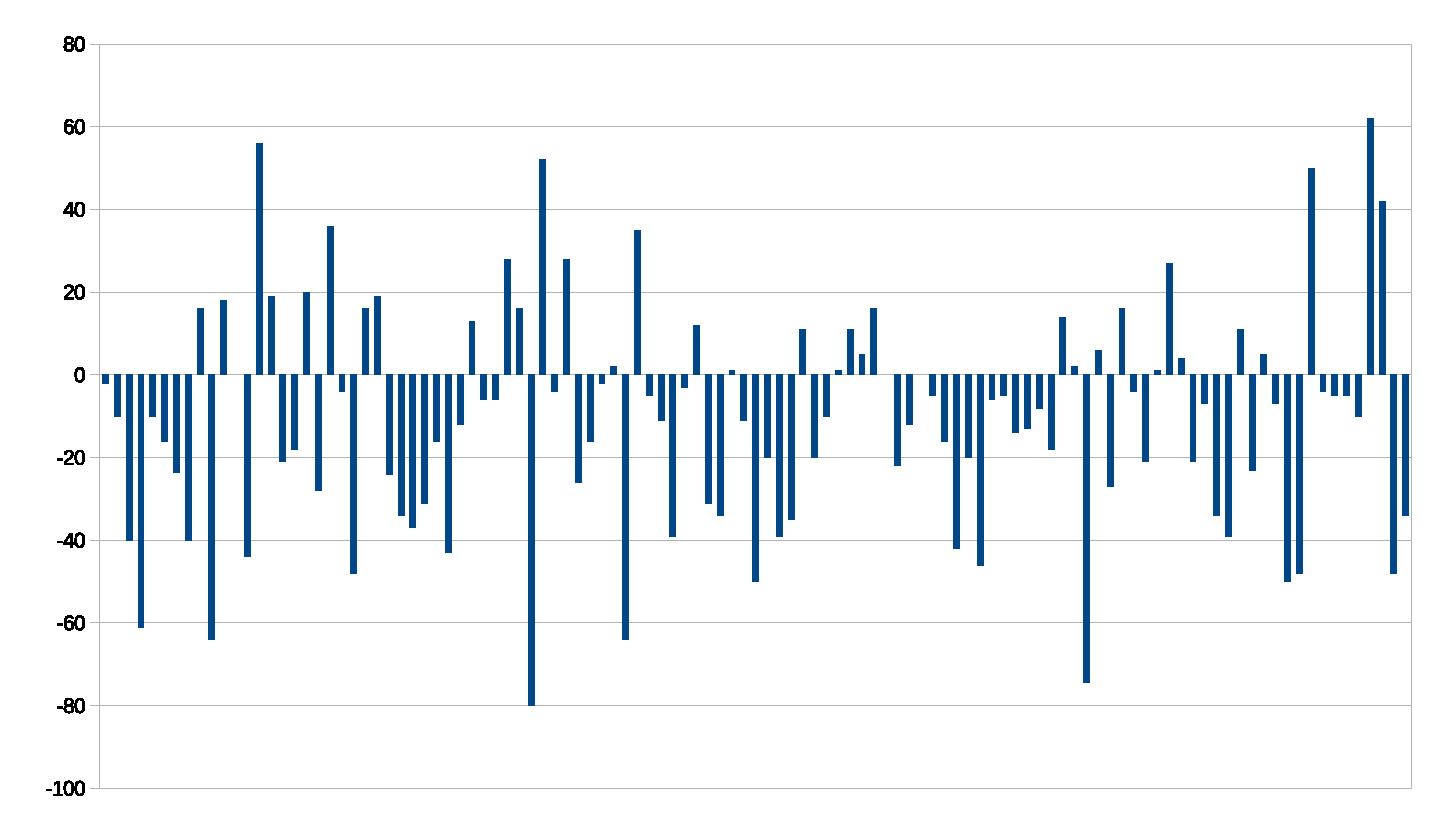
\includegraphics[width=9cm]{D_ma}
\caption{Saldos \texttt{TOTAL} actual del professorat any 2018}
\label{fig:1}
\end{figure}
\begin{figure}
	\centering
	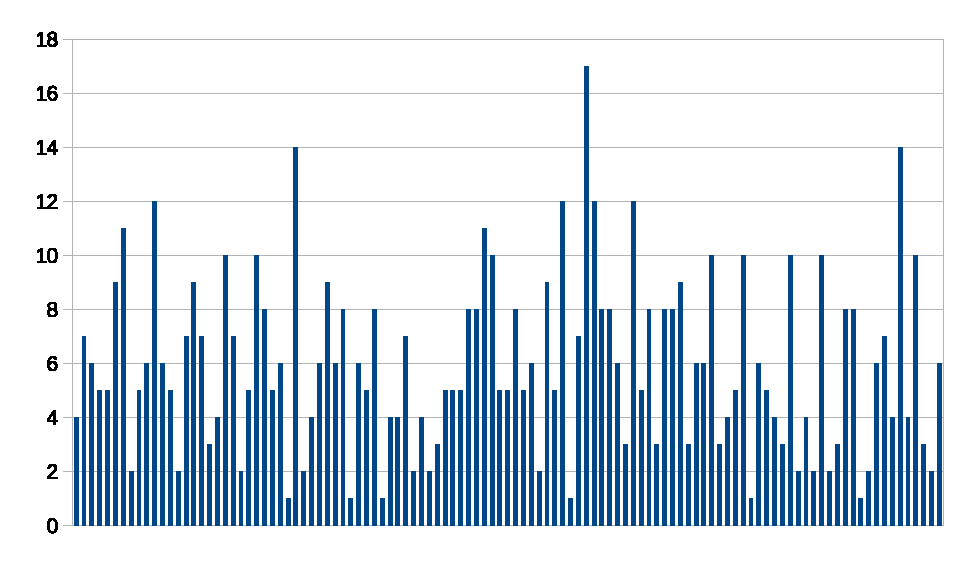
\includegraphics[width=9cm]{dis_ma}
	\caption{Dispersió \texttt{TOTAL} actual del professorat any 2018}
	\label{fig:2}
\end{figure}
\subsection{Conclusions}
		\begin{enumerate}
		    \item La variància del \textit{Saldo} sembla ser \textit{millorable}.
			\item El model actual funciona prou bé, fixa normes generals i fa un tractament diferent per cada cas, aconseguint més satisfacció en les assignacions. Per tant podem aprofitar molt del model actual. 
			\item Les particularitats \textit{bones} del model, entre altres, són el tractament prou adaptable a la \textit{diversitat} del professorat.
			\item Els aspectes negatius del model no són clars llevat de la \textit{alta} dedicació que requereix. La necessitat d' un temps de dedicació considerable per fer quadrar totes les assignacions satisfactòriament potser sembla ser un preu. \textit{massa alt}
			\item No analitzem la satisfacció del professorat amb el model actual, però la considerem la \textit{millor} fins el moment. 
		\end{enumerate}
\newpage
$\esp$
\newpage
%%%%%%%%%%%%%%%%%%%%%%%%%%%%%%%%%%%%%%%%%%%%%%%%%%%%
%                   Model d'optimització o        %%
%    #03                                          %%
%                 investigació Operativa          %%
%%%%%%%%%%%%%%%%%%%%%%%%%%%%%%%%%%%%%%%%%%%%%%%%%%%%
\begin{tcolorbox}[colframe=white,colback=redviolet!20,sharp corners=all,size=minimal,halign=center,valign=center]
\section{Model d'Optimització o d'investigació operativa}
\end{tcolorbox}
\lettrine{U}na altra forma d'abordar el problema és començar definint què és una \textbf{alternativa bona}, donant una mesura explícita de com de bona és una \textbf{alternativa}, és a dir, com de satisfactòria és una assignació d'assignatures entre el professorat.

Fins ara s'utilitzava una mesura no definida basada en el \textit{coneixement implícit} del sistema que tenia el professor que realitzava l'assignació. Donat $I$ el conjunt finit de professors i $o \in N$ el nombre d'assignatures que s'han de distribuir, definim la mesura mencionada com una funció:

$$F: I^o \longrightarrow \R$$

tal que com \textit{més baix} sigui $F(a)$ (donat $a \in I^o$) millor serà l'alternativa $a$.

Un cop haguem trobat una funció que compleixi això, trobar una alternativa bona passarà a ser un problema d'optimització, el qual tractarem amb una filosofia \textbf{heurística} a la secció 3.2 (Optimització).

És a dir, farem servir la \textit{típica estratègia} elemental d' investigació d'operacions:
\vspace{3 mm}

\begin{tcolorbox}
	\texttt{\textbf{maximitzar} o \textbf{minimitzar}} \texttt{F}
	\\ 
	\texttt{Subjecte a:}
	\\
	\text{ } \hspace{10mm} \texttt{\textbf{restriccions}}
\end{tcolorbox}
En aquest cas, \textbf{minimitzarem} la funció $F$ encara a definir.
\vspace{3mm}

\subsection{Definició o Ontologia de la funció objectiu}
Determinar la \textbf{funció objectiu} resulta inevitablement difícil, ja que aquesta està lligada al criteri subjectiu de cada professor. Malgrat això, podem aplicar diverses \textbf{restriccions} sobre les  \textbf{alternatives} que estan \textit{prohibides} pel sistema (com per exemple: un professor assignat a dos classes que es realitzin simultàniament), de manera que ens aquests casos la funció donarà infinit o bé els descartara. En els altres casos, en els que hem de determinar la qualitat d'una \textbf{alternativa factible} ens trobem amb l'ambigüitat que havíem comentat anteriorment, ja que per cada professor aquesta funció seria diferent i hem de balancejar els desitjos d'uns professors amb els dels altres, ja que en molts casos ens trobarem que una \textbf{alternativa} que és \textit{millor} per a uns, és \textit{pitjor} pels altres. Hi ha diverses possibles sortides a aquesta problemàtica:
\begin{enumerate}
	\item \textbf{Basar-nos en dades Històriques} fent un recull del \textit{historial}  d'alternatives prèvies, juntament amb les dades base que es van utilitzar per crear-les, podem intentar trobar la \textbf{funció implícita} que es va utilitzar per \textit{avaluar} les \textbf{alternatives}. És a dir, buscar, utilitzant aproximacions de funcions, una funció sobre les \textbf{dades base} \footnote{De nou aquestes estarien basades en l'historial recuperable, d'almenys,cinc anys enrere.} tal que, al optimitzar-la sobre cada un dels conjunts de dades base de cada any, doni una \textbf{alternativa} el més semblant possible a la solució que es va utilitzar aquell any. 
	\item \textbf{Obtenció de dades mitjançant enquesta} preguntant als professors directament què valoren més i creant una funció de forma artesanal basant-nos en els resultats.
	\item \textbf{Funcions personalitzables} a nivell individual per cada professor. A partir d'aquestes funcions individuals podem crear una funció global que estigui formada per un sumatori d'aquestes funcions tal que al optimitzar aquesta funció global estarem optimitzant les funcions individuals en conjunt. Això a la pràctica és pot traduir en contemplar tots els criteris a la vegada i en cas de que un criteri estigues més present augmentar-ne el \textit{pes} en la \textbf{funció objectiu} $F$.
\end{enumerate} 
\begin{figure}
	\centering
	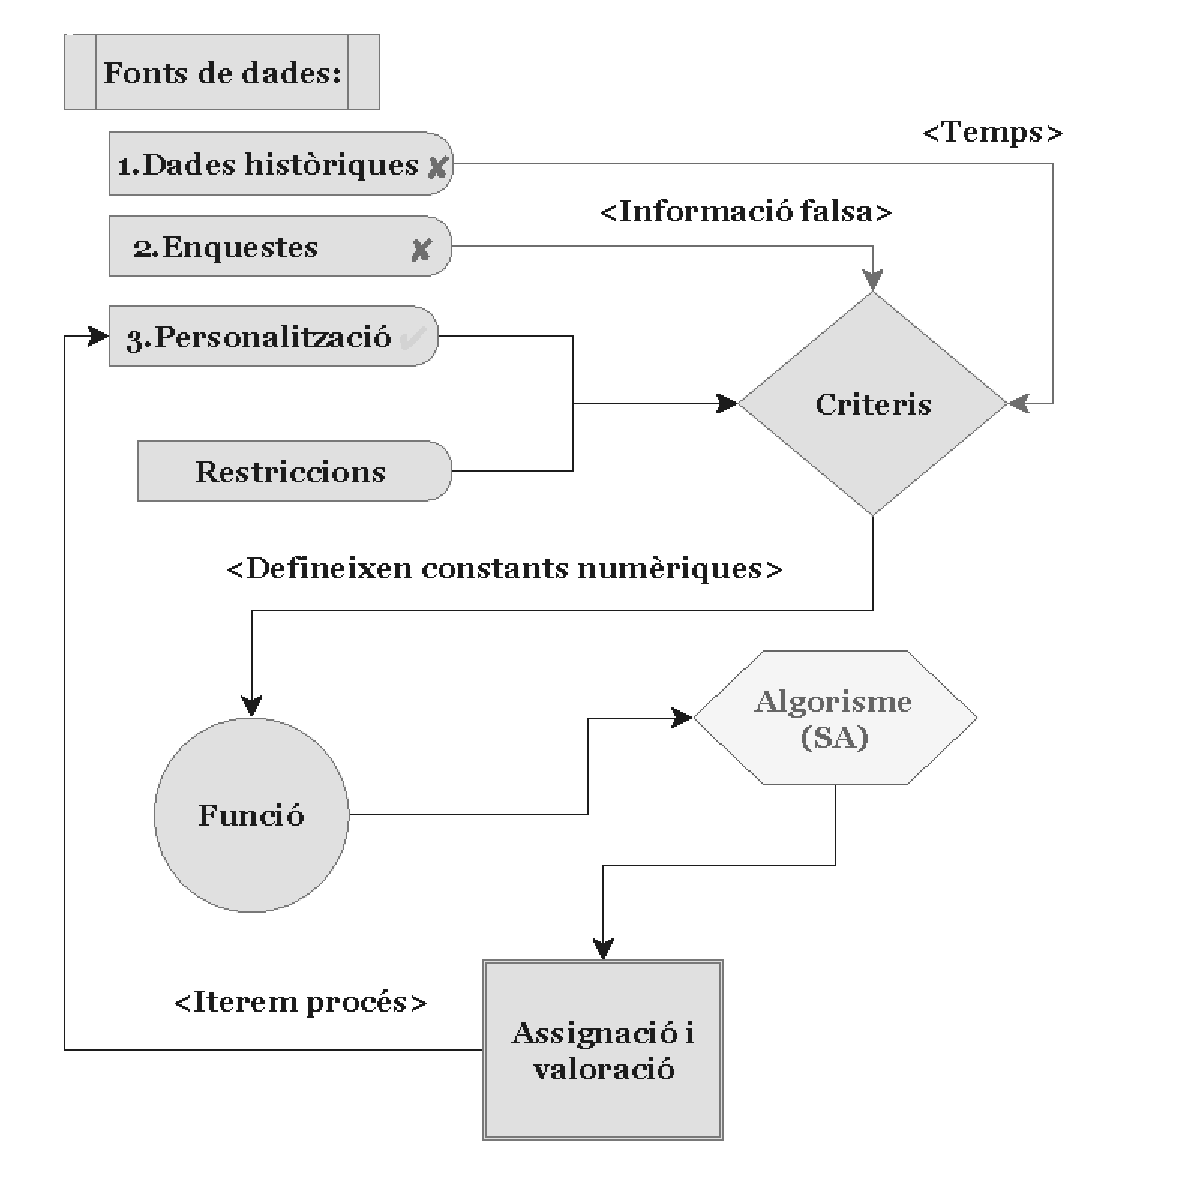
\includegraphics[width=9cm]{algor_bl}
	\caption{ \footnotesize Esquema que il·lustra les diferents \textit{vies} que és podrien considerar a l'hora de concretar aquesta funció $F$ que valores \textit{com de bona}  és una assignació d'assignatures entre el professorat. El \textit{hexàgon irregular}   (en un color més clar) representa un algoritme d'optimització concret. Simulated annealing, o de forma abreujada (SA), té origen en l'industria metal·lúrgica i està pensat per buscar \textbf{solucions optimes} en \textit{espais de cerca} grans. La seva presencia és \textit{oportunista} però no compromet la idea general ja que podríem encaixar, en el mateix esquema, qualsevol altre algorisme d'optimització, cosa que farem en la subsecció 3.5 ( resultats del model).}
	\label{fig:4}
\end{figure}
A la figura \ref{fig:4} observem un esquema que il·lustra la problemàtica i els tres punts esmentats on  l'\textit{idea clau} és respondre la pregunta.
\vspace{1mm}

\textit{Com justifiquem que els criteris que fixem i definiran la funció són bons o es corresponen amb el desig del professorat ?} 
 
\vspace{1mm}
En el nostre cas \textit{apostem} per un \textit{mix} entre el punt 2 i 3. Personalització limitada per restriccions, però adaptable a les \textit{particularitats} del Departament i les \textit{preferències}. La idea és facilitar una \textit{Biblioteca} de funcions per definir la funció final com a la suma d'una selecció d'aquestes.

\subsection{Ventall de criteris i Biblioteca de \textit{subfuncions}}
Definirem de forma additiva la funció $F$, és a dir, direm com es pot construir a partir d'altres \textit{subfuncions} i perquè ho fem així. Amb notació anterior tenim:

$$
\begin{matrix}
F: I^o \longrightarrow \R \qquad \quad  \\
a\longmapsto \displaystyle \sum_{i=1}^{k}f_i(a) \\
\end{matrix}
$$
On cada $f_i$ representa un \textit{criteri matematitzat} que  valora un aspecte concret. D'aquesta manera podem fer que la funció tingui en compte tants criteris com vulguem i que el fet de \textit{suprimir-ne} un  o \textit{afegir-ne} un altre no impliqui definir de nou la funció.
Això respon \textit{fortament} a {\color{violet!60}$\blacksquare$}$^{(05)}$.

La pregunta ara doncs és: \textit{Quina mena de funcions podem donar ?} De fet aquesta pregunta és massa ambiciosa, però donem alguns del exemples de funcions que hem vist \textit{raonables} i \textit{interessants}, i a més poden facilitar la tasca. De fet d'ara en endavant ens referirem a un conjunt de \textbf{subfuncions} concretes com a \textbf{Biblioteca}.
\vspace{3mm}

\begin{itemize}[$\RHD$]
	\item \begin{tabular}{|c|m{50mm}|}
		\hline
		\textbf{Criteri (B:1):}& Moderar el nombre d'assignatures  per professor.\\
		\hline
		\textbf{Funció (B:1):}& $\begin{matrix} \\ f_1(x)=x^3 \\ \\ \end{matrix}$\\
		\hline
		\textbf{Comentari (B:1):}& Aconseguir minimitzar el nombre d'assignatures que fa cada professor. Si volem ficar més pes només hem d'augmentar el grau del \textit{monomi}.\\
		\hline
	\end{tabular}
   \vspace{3mm}
    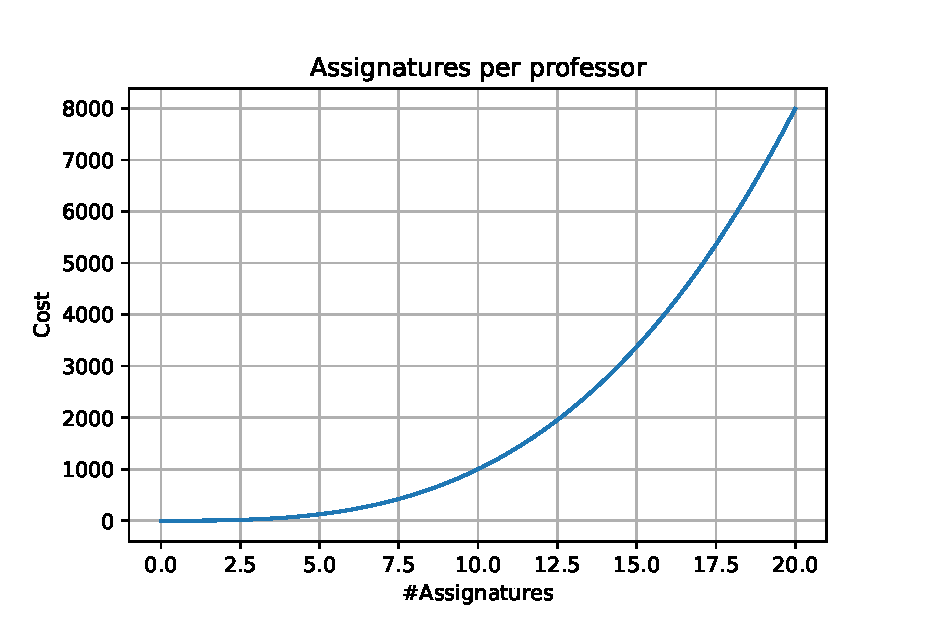
\includegraphics[width=8.5cm]{asig_mf}
    \\ 
    {
    \textbf{Figura (B:1):} 
    {\footnotesize Gràfic de la funció $f_1(x)=x^3$.}}
\vspace{3mm}
\item 
\begin{tabular}{|c|m{5cm}|}
	\hline
	\textbf{Criteri (B:2):}& Limitar el nombre d'hores de classe per dia.\\
	\hline
	\textbf{Funció (B:2):}& \footnotesize $\begin{matrix} \\ f_2(x):=\left\lbrace 
	\begin{matrix}
		(x-500)^2& \text{ si}& x>500\text{ ,} \\
		0& \text{ si}& x\leq 500& \end{matrix}
	\right.\\ \\ \end{matrix}$\\
	\hline
	\textbf{Comentari (B:2):}& La funció a trossos contínua penalitza \textit{fortament} qualsevol assignació que faci que un docent hagi de fer més de 500 min de classe en un dia. \\
	\hline
\end{tabular}
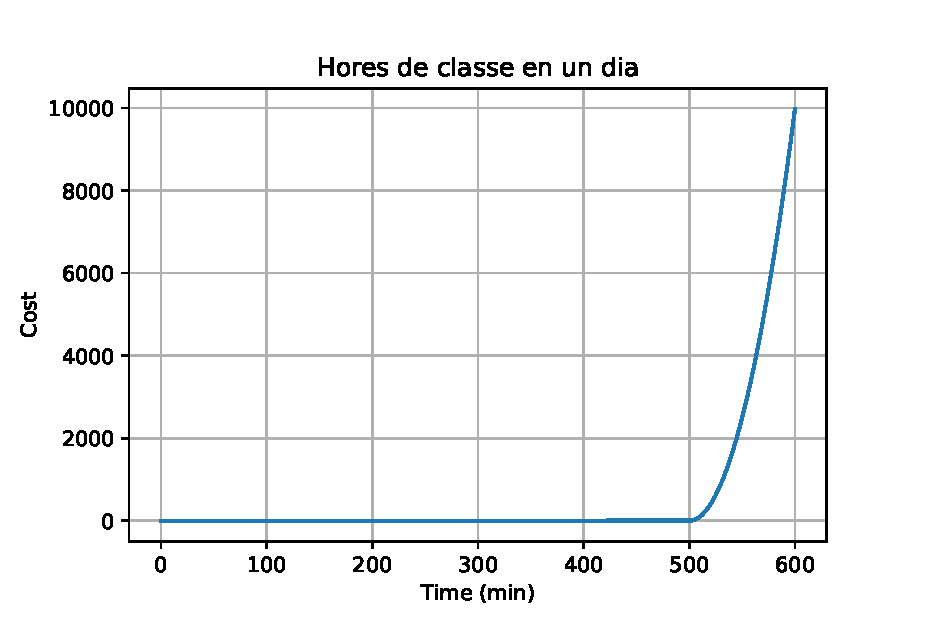
\includegraphics[width=8.5cm]{timeday_mf}
\\ 
{
	\textbf{Figura (B:2):} 
	{\footnotesize Gràfic de la funció  $f_2(x):=\left\lbrace 
		\begin{matrix}
			(x-500)^2 \text{ si } x>500\text{ ,} \\
			0  \qquad \qquad \text{ si } x\leq 500\end{matrix}
		\right.\\ $.}}
\item \begin{tabular}{|c|m{50mm}|}
	\hline
	\textbf{Criteri (B:3):}& Moderar els saldos molt alts en valor absolut.\\
	\hline
	\textbf{Funció (B:3):}& $\begin{matrix} \\ f_3(x)=x^2 \\ \\ \end{matrix}$ \\
	\hline
	\textbf{Comentari (B:3):}& Agafant la noció de \textit{saldo} del \textbf{model actual}. La idea és aconseguir que no hi hagi saldos molt \textit{grans}, ja que d'aquesta forma aconseguim adequar les hores que ha de fer cada professor o professora a la llarga. També evitem la acumulació de \textit{deutes} que a la llarga serien \textit{insalvables}.\\
	\hline
\end{tabular}
    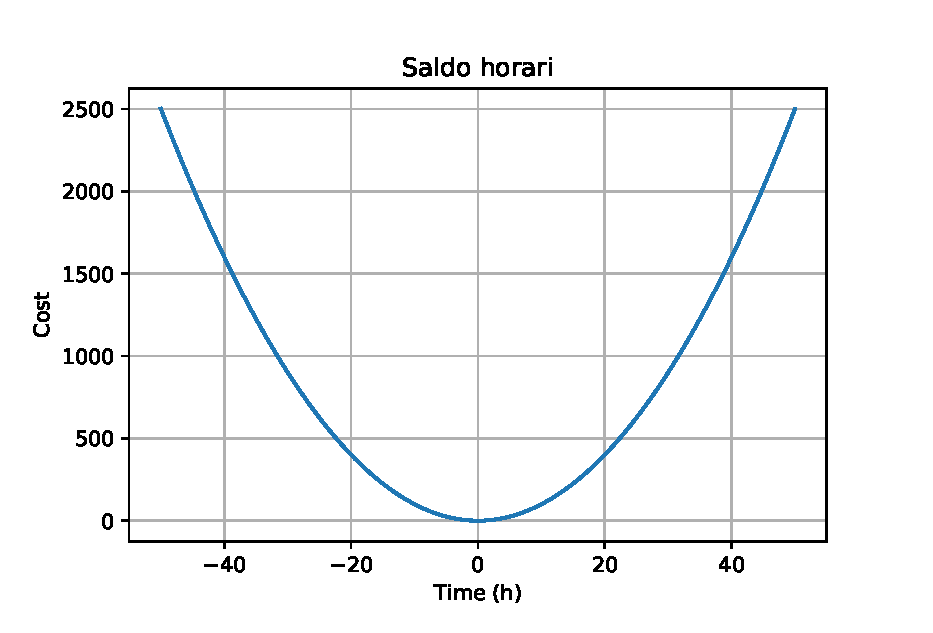
\includegraphics[width=8.5cm]{D_mf}
    \\ 
    {
	\textbf{Figura (B:3):} 
	{\footnotesize Gràfic de la funció $f_3(x)=x^2$.}}
\\
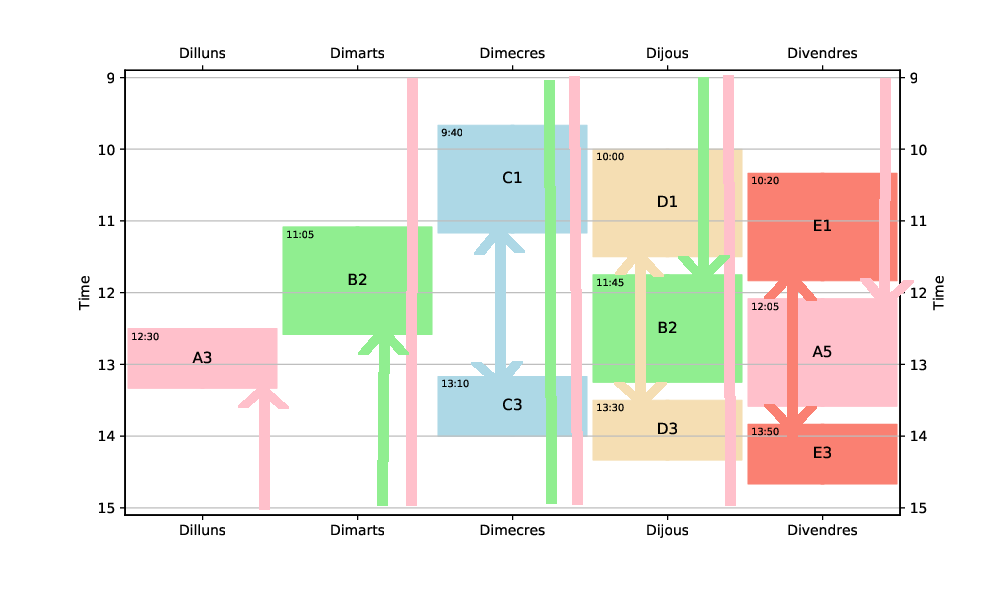
\includegraphics[width=8.5cm]{inter_mf} 
{\textbf{Diagrama (B:4):} {\footnotesize Diagrama que il·lustra  la distància \textit{en temps} entre les hores de classe de diferents docents (cada color representa un docent) on les fletxes (en el mateix color, diferent per cada docent) il·lustren la distància entre les assignatures que han d'impartir  en diferents dies d'una setmana.}}
\item \begin{tabular}{|c|m{50mm}|}
	\hline
	\textbf{Criteri (B:4):}& Temps entre classes \textit{desagradables} o \textit{inviables}.\\
	\hline
	\textbf{Funció (B:4):}& \footnotesize
	 $\esp$
	 
	 $f_4(x):=$
	 
	 $\esp$
	 
	 
	$\begin{cases}
    \left(2\cdot(15-x)\right)^2 &\text{ si } 0 \leq x \leq 15 \\
     x-15 &\text{ si } 15 \leq x \leq 300\\
     30\log{\left(\cfrac{x}{300}\right)}+285 &\text{ si } 300 \leq x \\ 
      \end{cases}$
      
      $\esp$
	\\ 
\hline
	\textbf{Comentari (B:4):}& Aquest \textit{subfunció}  definida a trossos evita  temps \textit{inviables} entre classe. Com per exemple: acabar una classe i començar la següent de forma \textit{instantània} (Aquest seria l'us \textit{ics} quadrat); o bé temps molt distants (Evitant així casos com tenir  únicament dues assignatures  en un mateix dia separades potser per 5 hores $\approx 300 \esp min$).\\
	\hline
\end{tabular}
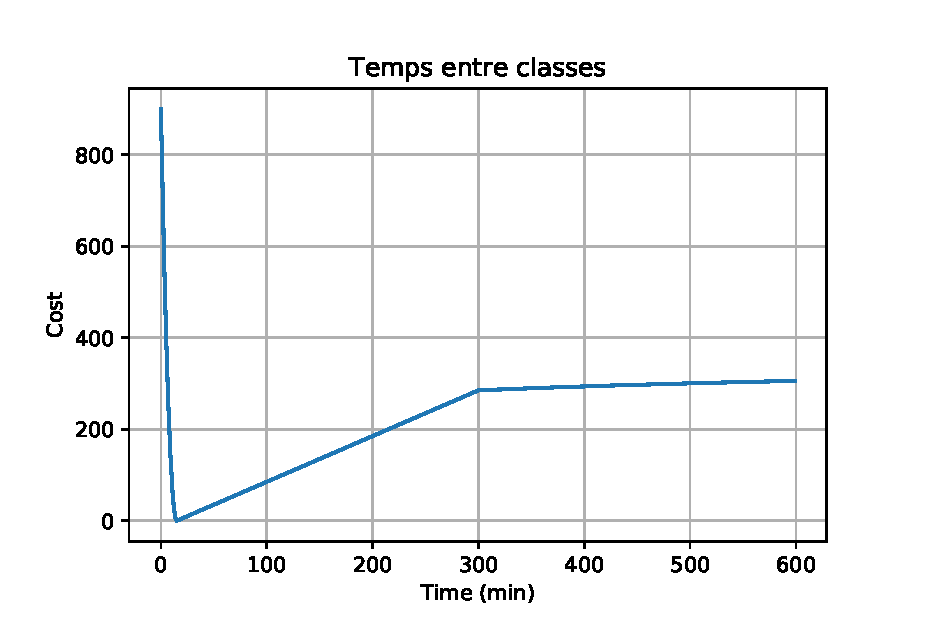
\includegraphics[width=8.5cm]{interc_mf}
\\ 
{
	\textbf{Figura (B:4):} 
	{\footnotesize Gràfic de la funció $f_4(x)$ definida a trossos.
		}}
\end{itemize}
\subsection{Optimització}
Optimitzar $F$ resulta un problema molt difícil, ja que tenim unes $\approx 100^{500}$ \textbf{alternatives} \footnote{Altrament $ \approx 10^{1000}$.} Inicialment vam utilitzar \textit{Simulated Annealing} (Algorisme d'Optimització apropiat per a grans \textbf{espais de cerca} ) amb control de mínims locals per tal d'optimitzar  la funció $F$ en un temps \textit{raonable}. Però, donada la \textit{filosofia} del treball, vam voler  optimitzar la \textbf{funció objectiu} de forma pròpia mitjançant selecció d'algoritmes genètics.   
\begin{enumerate}
	\item \textbf{Simulated Annealing:} Algorisme  basat en el mètode de Montecarlo \textit{refinat}, és apropiat per \textbf{espais de cerca} grans. Té origen en una tècnica de l'industria metal·lúrgica i es sol aplicar en \textit{optimització}.
	\item \textbf{Algorisme genètic:} Els algoritmes genètics, els quals es basen en el procés evolutiu, de forma molt simplificada consisteixen en generar solucions per a un problema mitjançant la recombinació de solucions anteriors i l'aplicació de mutacions aleatories sobre la solució, per després evaluar les solucions obtingudes i elegir les millors, millorant respecte les \textit{solucions anteriors} i imitant així la \textit{selecció natural biològica}.
	\item \textbf{Altres algorismes d'optimització de funcions no lineals meta-heurístics:} També és podrien haver fet servir algorismes com:  
	\begin{enumerate}
		\item Optimització d'eixam de partícules
		\item Cerca de cucut
		\item Cerca de tabus
		\item Algorisme de cerca gravitativa
		\item Túnels estocàstics
		\item Optimització de colònies d’abelles artificials
		\item Recuit simulat
		\item Túnels estocàstics
	\end{enumerate}
\end{enumerate}
\subsection{Limitacions del model}
És clar que en primera instancia una estratègia prou pràctica com els \textit{algorismes} per optimitzar el model es podria tirar per terra argumentant que cap d'aquest mètodes (\textit{simulated annealing} i \textit{Algorismes genètics}) podran trobar el mínim absolut de la funció a optimitzar $F$. 

Un argument així no \textit{correspon} amb la \textit{filosofia del treball}. Això no ens resulta problemàtic, ja que només ens cal que la \textbf{solució} sigui \textit{bona}, entenent com a bon que sigui: \textbf{factible} , que consumeixi un temps \textit{raonable} en ser trobada i que sigui \textit{substancialment millor} que la del \textbf{model actual}. I això és pot comprovar fàcilment com farem en la subsecció de 3.5 Resultats.

De fet només hem donat una \textit{definició constructiva}, és a dir, hem donat una \textit{idea} de com construir $F$, però no l'hem explicitat ja que la \textit{màgia} d'aquesta és que es pugui adaptar a restriccions i criteris diferents. Cosa que respon \textit{fortament} a  {\color{green!60}$\blacksquare$}$^{(03)}$, {\color{cyan!60}$\blacksquare$}$^{(01)}$ i {\color{violet!60}$\blacksquare$}$^{(05)}$.
\subsection{Resultats del model}
Els resultats més rellevants d'aquest model són:
\begin{enumerate}
	\item Possibilitar la cerca de \textbf{solucions factibles}\footnote{Enteses com a assignacions que compleixen amb les \textbf{restriccions} imposades. }
	\item Possibilitat de millorar optimització d'alguns aspectes del \textbf{model actual}.
\end{enumerate}
Comparant aquest model, \textbf{model d'investigacions operatives}, amb el \textbf{model actual} agafant com a \textbf{funció objectiu} :
$$
F=\sum_{i=1}^{2}(f_i)(a) 
$$
$$\text{ amb } \qquad f_1(a)=\sum_{j=1}^{111} (x_j-x'_j)^2 \qquad \text{ i }$$  
on $x_j$ serien les hores de classe que hauria de fer un professora o professor $j \in \{1,\cdots,111\}$ i $x_j'$ les hores que farà amb l'assignació $a$ el professor $j \in \{1,\cdots,111\}$.
$$\text{ amb }  \qquad f_2(a)=\sum_{j=1}^{111} (y_j)^3$$
on $y_j$ serien el nombre de matèries docents que hauria de fer un professor $j \in \{1,\cdots,111\}$   amb \textbf{alternativa} $a$. 

Això seria el que actualment s'intenta minimitzar. Programant en Python (amb els dos algorismes per \textit{minimitzar}) obtenim els resultats que es veuen en les figures 4 i 5 (per el saldo); i 6 i 7 (pel nombre d'assignatures).
Resumint aquestes podem observar Taula 1. 
\vspace{3mm}

\begin{tcolorbox}[colback=white,coltitle=black,colframe=white, colback=white]
{\centering
	\small
	\begin{tabular}{|c|c|c|c|}
	\hline
     \textbf{Model}&\textbf{actual}&\textbf{$F$+(SA)}&\textbf{$F$+(GA)}\\
     \hline
     Variància&737'0676&14'7221&124'70397\\
     \hline
     Suma absoluta&2498&1156&1461\\
     \hline
	\end{tabular}
}
\end{tcolorbox}
\noindent \textbf{Taula 1:} \small{Suma del valor absolut dels saldos dels professors  i la seva variància, tant del \textit{model actual} (primera columna), com dels models d'optimització de $F$ tant amb \textit{Simulated annealing} (tercera columna) com amb \textit{algorismes genètics} (quarta columna).}
\vspace{3mm}

\normalsize
Concloem doncs que els models d'optimització donen una \textbf{solució bona}. Es milloren els resultats del \textbf{model actual}.
	\begin{figure}[!]
		\centering
		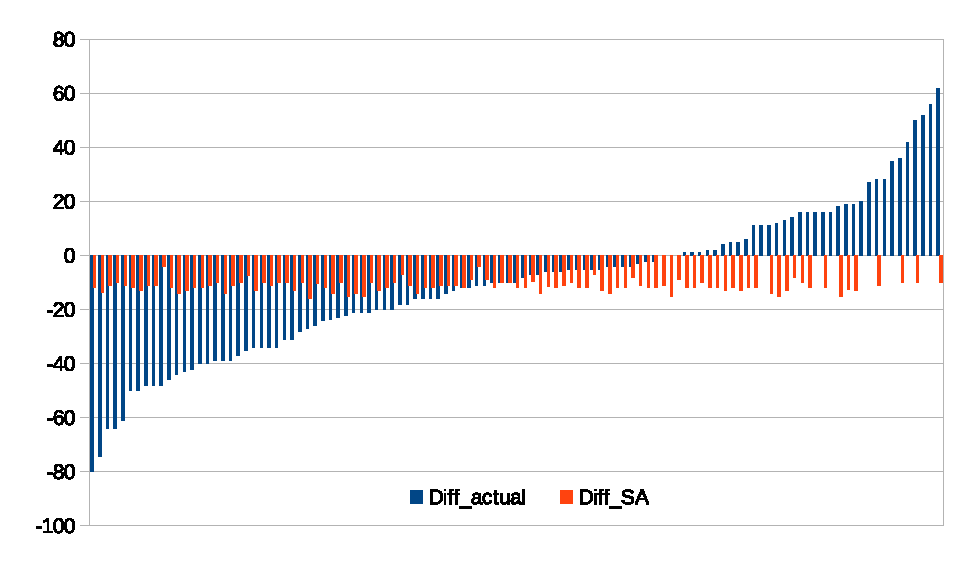
\includegraphics[width=9cm]{sorted_mo}
		\caption{ \small Saldo \texttt{TOTAL}  del professorat en l'any 2018 amb ({\color{blue!70}$\blacksquare$}) \textit{model actual}  i ({\color{orange!70!red!90}$\blacksquare$}) \textit{model Optimització amb SA} (Simulated annealing). Cada columna representa el saldo d'un professor, les columnes han sigut ordenades de més petita a més gran tenint en compte el signe, respecte el \textit{model actual}. }
		\label{fig:6}
	\end{figure}
	\begin{figure}[!]
		\centering
		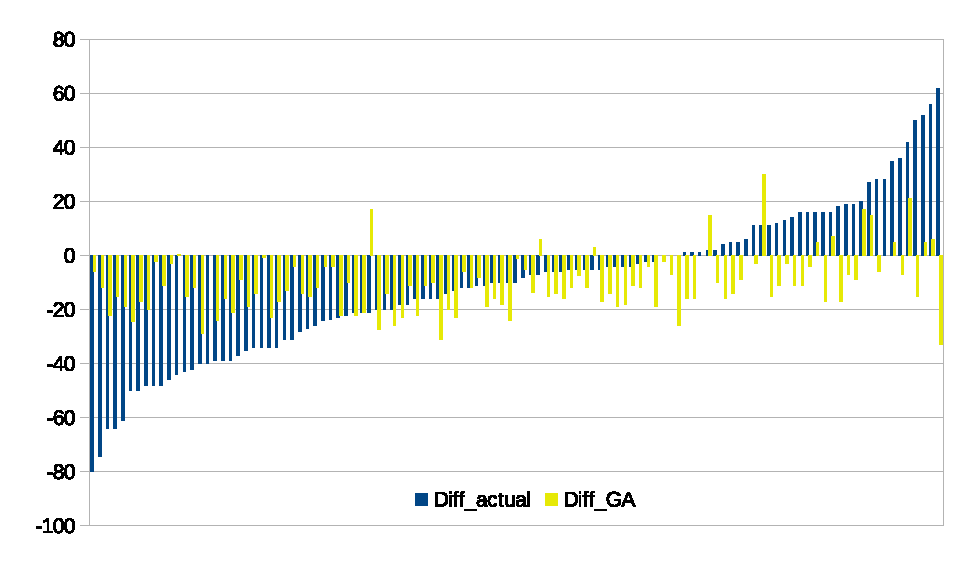
\includegraphics[width=9cm]{sorted2_mo}
		\caption{ \small Saldo \texttt{TOTAL}  del professorat en l'any 2018 amb ({\color{blue!70}$\blacksquare$}) \textit{model actual}  i ({\color{yellow!70!gray!90}$\blacksquare$}) \textit{model Optimització amb GA} (Algorismes genètics). Cada columna representa el saldo d'un professor, les columnes han sigut ordenades de més petita a més gran tenint en compte el signe, respecte el \textit{model actual}. }
		\label{fig:64}
	\end{figure}
	\begin{figure}[!]
		\centering
		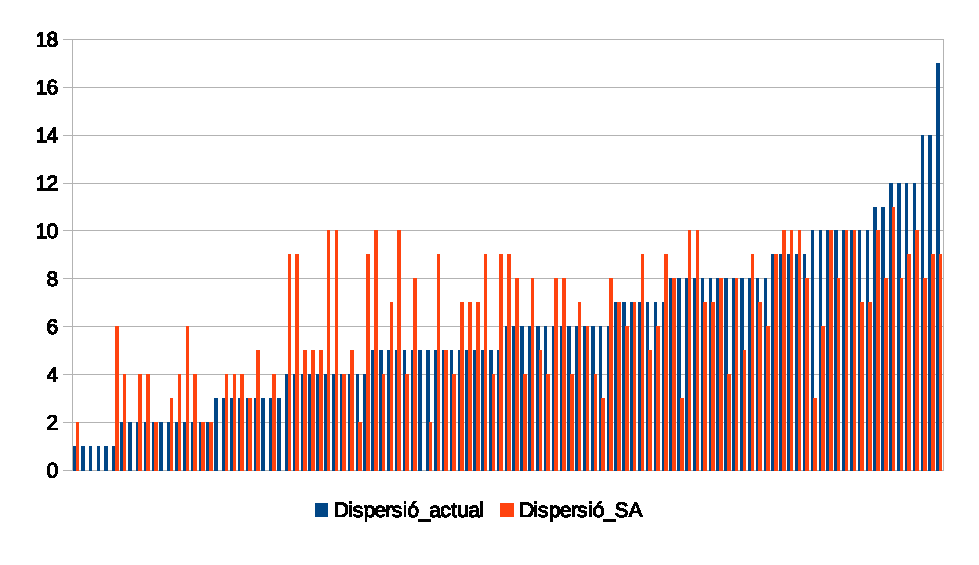
\includegraphics[width=9cm]{disp_sorted_sa}
		\caption{ \small Nombre \textit{d'assignatures} que fa el professorat en l'any 2018 amb  ({\color{blue!70}$\blacksquare$}) \textit{model actual} i ({\color{orange!70!red!90}$\blacksquare$}) \textit{model Optimització amb SA} (Simulated annealing). Cada columna representa el nombre d'assignatures que fa un docent, les columnes han sigut ordenades de més petita a més gran tenint en compte el signe, respecte el \textit{model actual}. }
		\label{fig:sor}
	\end{figure}
	\begin{figure}[!]
		\centering
		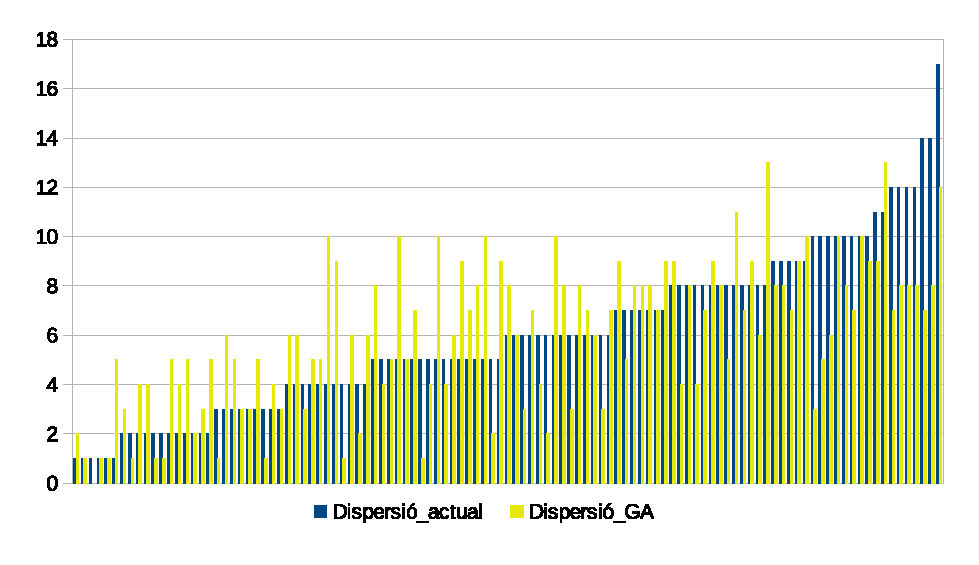
\includegraphics[width=9cm]{disp_sorted_ga}
		\caption{ \small  Nombre \textit{d'assignatures} que fa el professorat en l'any 2018 amb  ({\color{blue!70}$\blacksquare$}) \textit{model actual} i ({\color{yellow!70!gray!90}$\blacksquare$}) \textit{model Optimització amb GA} (Algorismes genètics). Cada columna representa el nombre d'assignatures que fa un docent, les columnes han sigut ordenades de més petita a més gran tenint en compte el signe, respecte el \textit{model actual}. }
		\label{fig:sorted_mo}
	\end{figure}
\newpage
\subsection{Alguns detalls sobre el procés d'elaboració dels algoritmes genètics}
\normalsize
Com hem explicat a l'apartat 3.3, els algoritmes genètics generen possibles \textbf{solucions} a base de recombinar i mutar solucions ja existents\cite{ga}. Aquests mecanismes abstractes, així com la codificació de la solució sobre la qual operen, admeten moltes possibles variacions, les quals s'han d'adaptar al problema per aconseguir el \textit{màxim rendiment}.

En la nostra implementació dels algoritmes genètics, hem optat per representar el fenotip (la codificació de cada solució generada) com una matriu de professors, on cada posició defineix quin professor es assignat a cada assignatura diferent. La mutació es implementada com una assignació d'una assignatura aleatòria a un professor aleatori; per altra part la recombinació crea noves solucions a partir de dos solucions triades aleatoriameant entre les millors (la élit), generant una nova solució que tingui part de les assignacions d'assigatures d'una i part de l'altra. Altres parametres, com la mida de la població, la probabilitat de recombinació o la de mutació, s'han triat de forme empírica a base d'executar l'algorisme i buscar les constants que donaven els millors resultats.

A més a més, el nostre algoritme utilitza elitisme, de manera que les millors solucions són conservades entre iteracions de l'algorisme, portant a que noves generacions sempre millorin la funció de cost.

En la nostra implementació dels algoritmes genètics, hem optat per representar el \textbf{fenotip} (la codificació de cada solució generada) com una matriu de professors, on cada posició defineix quin professor es assignat a cada assignatura diferent. La \textbf{mutació} es implementada com una assignació d'una assignatura aleatòria a un professor aleatori; per altra part la recombinació crea noves solucions a partir de dos solucions triades aleatoriameant entre les millors (la \textbf{élit}), generant una nova solució que tingui part de les assignacions d'assigatures d'una i part de l'altra. Altres paràmetres, com la mida de la població, la probabilitat de recombinació o la de mutació, s'han triat de forme empírica a base d'executar l'algorisme i buscar les constants que donaven els millors resultats.

A més a més, el nostre algoritme utilitza \textit{elitisme}, de manera que les millors solucions són conservades entre iteracions de l'algorisme, portant a que noves generacions sempre millorin la funció de cost.

Comparant els resultats obtinguts en l'optimització en que hem utilitzat \textit{Simulated Annealing} i en la d'Algoritmes Genètics, és trivial veure que els resultats de SA són molt millors, ja que s'assoleixen assignacions amb diferències d'hores més ben distribuïdes. Aixó és així perquè hem executat els algoritmes durant poc temps (menys de 20 minuts) i el fet que les iteracions en GA són molt més lentes ha portat a que no s'aconseguís arribar a un mínim local.

Creiem que en d'executar l'algoritme durant períodes de temps més llargs, les capacitats per evitar mínims locals dels GAs mitjançant l'especiació portaran a una millora de resultats respecte al SA, ja que l'exploració realitzada pel GA cobrirà molt més \textbf{espai}.

\begin{figure}[!]
	\centering
	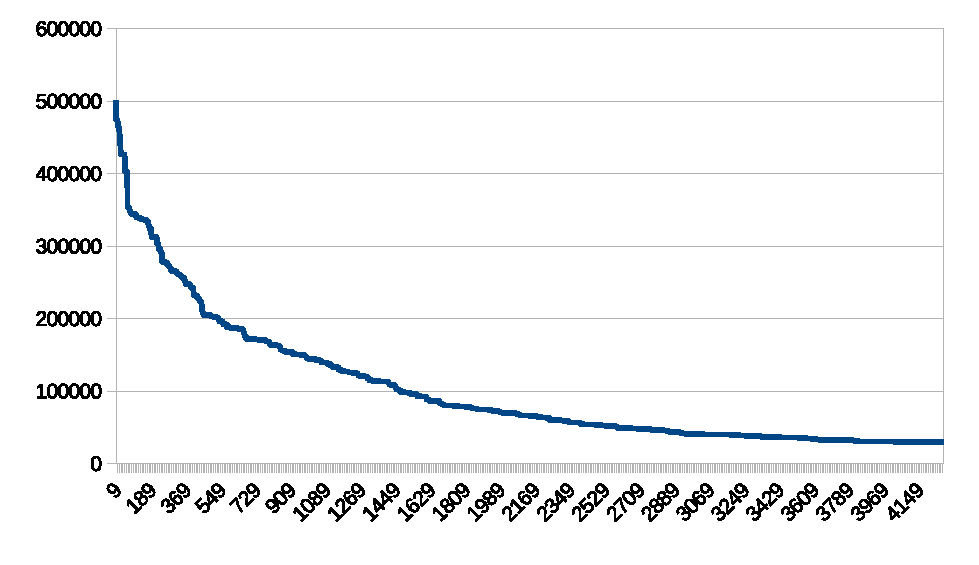
\includegraphics[width=9cm]{progress_ga}
	\caption{ \small Gràfica de l'evolució de la qualitat de la millor assignació de cada generació respecte al temps acumulat d'execució de l'algorisme genètic. }
	\label{fio}
\end{figure}
\begin{figure}[ht]
	\centering
	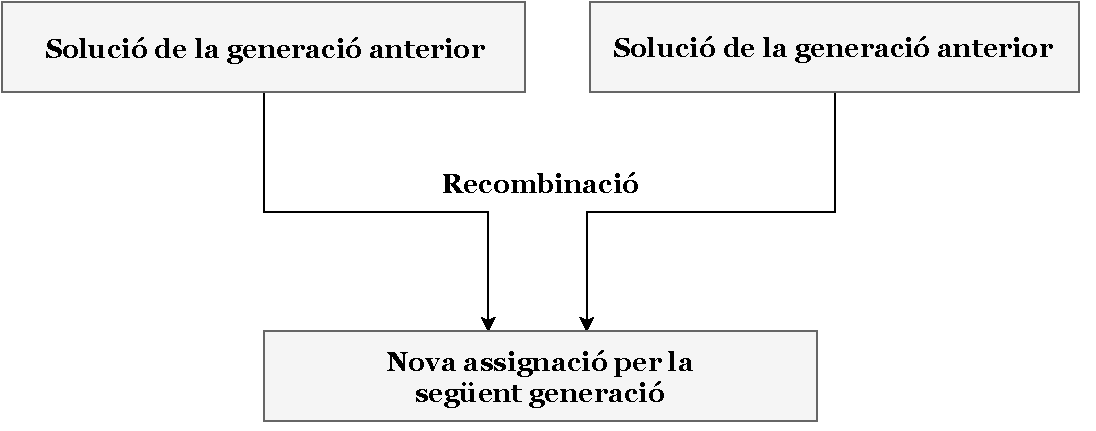
\includegraphics[width=9cm]{recombinacio}
	\caption{ \small Diagrama que il·lustra l'aplicació de l'operador de recombinació. }
	\label{firo}
\end{figure}
\subsection{Revalorització d'assignatures}
Durant l'optimització, els models actuals ja revaloritzen les assignatures de forma íntrinseca per tal d'aconseguir que la satisfacció de tots els professors sigui màxima. No obstant, ens interessa obtenir una valorització explícita, ja que aquest es un dels requísits que ha de complir el model d'acord amb l'enunciat del treball.

Per tal d'obtenir aquesta valoració, intentarem extreure aquesta valoració íntrinsica que es realitza durant l'optimització basant-nos en una comparació entre l'avaluació de l'estat actual d'un professor i el de la resta de professors.

Així doncs, començarem separant l'avaluació de l'estat d'un professor del de la resta en la funció d'avaluació de una assignació. Això ho podem fer perque totes les funcions que formen part d'aquesta funció d'avaluació, que realment és un sumatori de les primeres funcions, són independents entre elles i s'apliquen sobre només un professor. D'aquesta manera, dividim la funció d'avaluació:
$$F(a)= \displaystyle \sum_{p\in professors} \sum_{f_i\in funcions} f_i(p) = $$
$$= \displaystyle \sum_{p\in professors} f(p)$$
On és trivial observar que:
$$f(p)=\sum_{i\in funcions} f_i(p)$$

A partir d'aquí podem aplicar $f$ sobre l'estat de tots els professors i obtenir la mitja $\mu$ i la desviació típica $\sigma$ de la distribució d'aquests valors. 

A continuació calculem els següents valors, que ens permeten obtenir una aproximació de com de bo és l'estat d'un professor respecte la resta. A més, al dividir per sigma, obtenim un valor adimensional que rectifica les unitats que estiguem utilitzant (de manera que utilitzar unitats amb valors molt grans o molt petits no afectarà funcionalment el resultat final) i ens normalitza el resultat respecte a la variancia de les dades, de manera que un resultat podrà ser molt alt només si es extremadament diferent a la resta de dades.

$$\phi(p)=\dfrac{f(p)-\mu}{\sigma}$$

Finalment, revaloritzem les assignatures amb el següent càlcul:

$$h_{nou_a}=h_{vell_a}(1+\phi(p)\alpha) \forall a \in A_p$$

on $A_p$ és el conjunt d'assignatures realitzades pel professor $p$, i $\alpha$ és un paràmetre constant modificable que serveix per a modificar la intensitat de la revalorització per tal que s'adapti al funcionament esperat pels usuaris.


\newpage
$$
\esp
$$
\newpage
%%%%%%%%%%%%%%%%%%%%%%%%%%%%%%%%%%%%%%%%%%%%%%%%%%%%
%                                                 %%
%    #04    Models d'assignacions  per subhastes  %%
%                                                 %%
%%%%%%%%%%%%%%%%%%%%%%%%%%%%%%%%%%%%%%%%%%%%%%%%%%%%
\begin{tcolorbox}[colframe=white,colback=redviolet!20,sharp corners=all,size=minimal,halign=center,valign=center]
	\section{Models d'assignacions per subhastes}
\end{tcolorbox}
\lettrine{E}n aquesta secció abordarem la problemàtica d'assignacions mitjançant l'estructura de subhasta, pensant, com en les seccions anteriors, en la seva aplicació final. La intenció  és construir un mètode sobre l'estructura de subhasta que permeti  donar solució al problema dels repartiments.
\subsection{Problemàtiques i beneficis de les subhastes}
Tots tenim una idea intuïtiva de subhasta.Més enlla de les conegudes subhastes de \textit{eBay}  ni'ha de molts tipus altres tipus, que no només poden ser classificades per un únic criteri sinó per molts. Explicitem algunes d'aquestes classificacions.

Les \textbf{subhastes simultànies o paral·leles} són aquelles que és \textit{resolen} a la vegada, és a dir, només cal un \textit{instant} per determinar els guanyadors. Per conta les \textbf{subhastes seqüencials } són aquelles que decideixen \textit{una per una}. 

Les \textbf{subhastes a cegues} són aquelles en que les puges que fa cada participant de la subhasta no són públiques, en canvi, en les \textbf{subhastes públiques} sí.

Les \textbf{subhastes a l'alça} són aquelles en les qui guanya el participant que ofereix el major preu, en canvi les \textbf{subhastes a la baixa}, són guanyades pel participant que  ofereix el menor preu. Un exemple d'aquesta ultima podria ser el preu mínim que està disposat a rebré un \textit{participant} per fer  una tasca.

L'objectiu principal de la majoria de \textbf{subhastes} és vendre \textit{objectes} al preu més alt possible (suposant que fossin subhastes a l'alça),és a dir, maximitzen el \textit{guany} però en un cas com en el de repartir les assignatures entre el professorat del departament d'una facultat això no té sentit, ni és un bon plantejament, ja que no hi ha objectiu de guany, sinó únicament de repartiment.

Per tant una subhasta típica no seria pas una bona solució al problema de repartiment. No obstant hi ha un tipus de subhasta que no maximitza el benefici de \textit{venedor} sinó dels \textit{participants}, és a dir, en maximitza \textbf{l'utilitat} d'aquests. 

Aquest tipus de subhasta, que de fet és l'única que farem servir tot i donar dos models completament diferents basats en subhastes, es coneixen com a subhastes de \textbf{Vickrey}. Les \textbf{subhastes de Vickrey} són subhastes  simultànies a a cegues on el guanyador d'una subhasta és qui ofereix el preu més alt (suposant subhastes a l'alça) pagant el preu de la segona puja més alta.

En Teoria de jocs es pot demostrar que aquests tipus de subhasta és totalment eficient, que tal com havíem dit abans maximitza l'\textbf{utilitat} dels participants i incentiva de fer pugues \textit{racionals}, és a dir, pagar el que és creu correcte o \textit{just}.   


\begin{figure}[!]
	\centering
	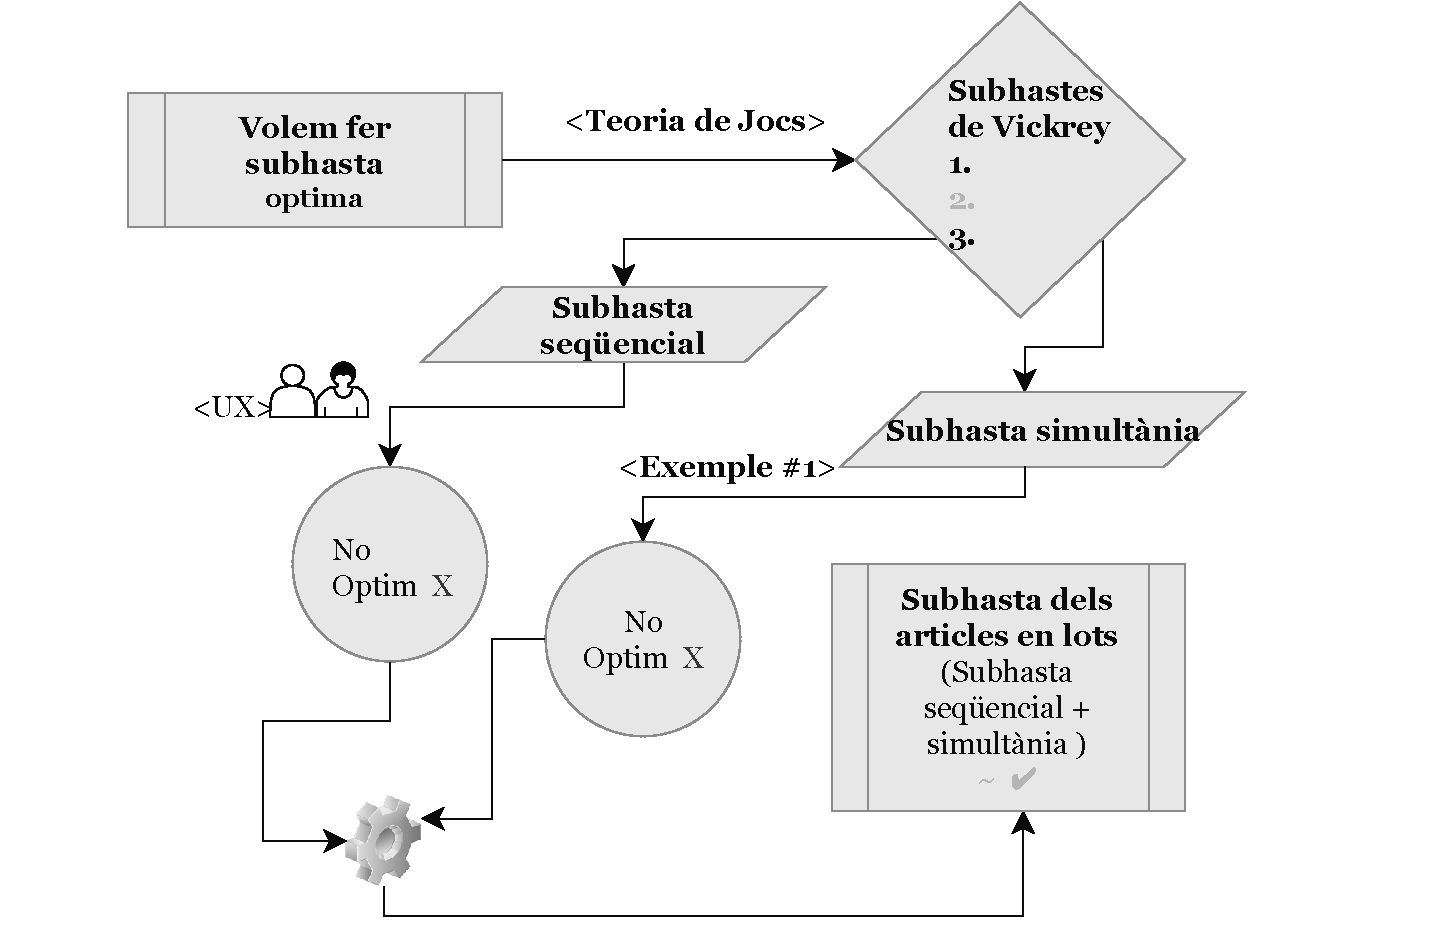
\includegraphics[width=9cm]{subs}
	\caption{ \footnotesize farem en la subsecció 3.5 ( resultats del model).}
	\label{fig:4}
\end{figure}
\subsection{Un model minimalista, els \textit{Kiwis}}
\subsubsection{Repartiment kiwis}
Per a tal de fer més justa la repartició d'assignatures i de premiar l'esforç del professorat i la qualitat de la seva feina, proposem un model de subhastes on la moneda de canvi, els kiwis, siguin repartits entre els pujadors de la següent manera:

Cada professor parteix de 10 Kiwis.
Si el professor té acumulat un saldo positiu (ha fet més hores del que li pertoquen en els ultims 3 anys) se li sumen 5 Kiwis per cada 10 hores que tingui en el saldo : 
\begin{itemize}
	\item 5 Kiwis per un saldo de 0 a 10h
	\item 10 Kiwis per un saldo de 11 a 20h
	\item  Etc.
\end{itemize}
A partir del segon any de l'instauració d'aquest model, si el professor va haver de impartir $x$ matèries que no va triar (assignades mitjançant la funció després de fer totes les subhastes) se li sumaran $x$ Kiwis. A aquells professors que vagin aconseguir més d'un 4.5 de mitjana en les enquestes realitzades per l'alumnat l'any anterior,  se li sumaran 30 kiwis. 

\subsubsection{Funcionament subhasta}
Realitzarem una subhasta per blocs de matèries, cada professor omplirà les caselles de les matèries per les que vulgui pujar d'un pdf amb el valor en kiwis que està disposat  a pagar. El preu inicial de cada matèria és de 0 Kiwis, la puja mínima és de 1 Kiwi, i a partir d'aquí es pot augmentar el preu de 0.5 Kiwis en 0.5 Kiwis (és a dir, les pujes vàlides per a una assignatura són: 1K, 1.5K, 2K, 2.5K, 3K,3.5K, etc.)

Un programa recullirà els resultats i otorgarà cada matèria al major pujador. En cas d'empat, es quedarà la matèria aquell professor qui partís de més kiwis al començament. En cas de tornar a haver empat, la assignatura quedarà lliure amb el valor obtingut com a valor inicial per a la següent subhasta.

D'aquesta manera es realitzaran tres subhastes. (En la última hi haurà la possibilitat de pujar amb Kiwis negatius: els pofessors poden oferir-se a fer una assignatura a canvi de rebre fins a 5 kiwis a canvi (pujant per -5 Kiwis)).

\subsubsection{Revalorització hores}

Suposem que tenim l'assignatura $A$ i volem revaloritzar-la en hores una vegada finalitzada la subhasta.
Suposem que durant la subhasta $x$ professors han pujat per l'assignatura i que el guanyador ha pagat $y$ kiwis per ella. Definim les següents funcions:

$$\varphi (x)=\frac{x}{x+a}\ ,\  \psi(y)=\frac{y}{y+b} \quad a,b\in\mathbb{R}^{+} $$
	
Llavors, per revaloritzar les assignatures proposem la següent formula:
$$h_f(x,y,h_0)=h_0(1-c_1\varphi(x)-c_2\psi (x))\esp ,\esp c_1,c_2\in\mathbb{R}^+$$
On $h_0$ és el nombre d'hores inicial en que està valorada una assignatura. Les constants $c_1,c_2$ són per donar-li més pes a una variable que a l'altra. La funció està dissenyada per tal de que la part que multiplica $h_0$ estigui acotada per $1$. Per tant s'ha de complir:
$$
c_1+c_2=1
$$
Cal triar doncs unes constants que reflecteixin la importància de cada una de les variables en la funció. Tenimen compte els següents fets per fer la tria:
\begin{itemize}
\item Que $y$ sigui gran no implica necessàriament que $x$ ho sigui. És a dir, que una assignatura es vengui per un valor elevat no implica que hi hagin molts professors interessats en ella. 
\item Contràriament, una $x$ gran sí que, per norma general, implicaria un valor de $y$ elevat.
\end{itemize}
Per tant, creiem que la variable $x$, i per conseqüència la funció $\varphi$ haurien de tenir més pes sobre la funció final ja que aquesta és en la qual es reflexa de millor manera L'interès que hi ha per una assignatura. Triem doncs les constants de les següent manera:
$$c_1=0.7\ ,\ c_2=0.3$$
Una vegada tenim les constants $c_i$ ens cal determinar $a,b$ de les funcions petites. Per fer-ho considerarem diversos casos concrets on tenim clar com hauria de ser la revalorització i prenem les constants que més ens satisfacin.
	\\
	Suposem doncs la següent situació que es la més habitual: Tenim la assignatura $A$ per la qual han pujat dues persones ($x=2$) i s'ha adjudicat per un preu de 5 kiwis ($y=5$). Aquesta, esta valorada inicialment amb 20 hores ($h_0=20$). Aquest valor inicial el posem basat en la mitjana de hores que acostuma a tenir una assignatura. Per tal de que la revalorització fos prou bona, el preu d'aquesta assignatura ha de ser dues terceres parts del valor inicial. Per tant, utilitzant la funció tindríem:
	$$20\cdot\frac{2}{3}=h_f(2,5,20)=20(1-0.7\frac{2}{2+a}-0.3\frac{5}{5+b})$$
	Sense oblidar-nos d'aquest cas, considerem-ne un de més conflictiu: Suposem que tenim una assignatura per la qual hem fet una puja 5 persones ($x=5$) i el preu final d'aquesta ha sigut de 10 kiwis ($y=10$) i valorada inicialment amb $10$ hores. Amb un preu tan alt i amb tants professors interessats en ella aquesta assignatura hauria de ser revaloritzada a 10 hores, Tenim doncs:
	$$10=h_f(5,10,20)=20(1-0,7\frac{5}{5+a}-0.3\frac{10}{10+b})$$
	Si resolem el sistema donat per les dues equacions anteriors obtenim:
	$$a=\frac{1}{5}\cdot (27+\sqrt{229})\approx 8.42$$
	$$b=\frac{1}{2}\cdot(111-7\sqrt{229})\approx 2.53$$
	Fent unes quantes proves concloem que aquestes constants ens donen resultats prou satisfactoris. Per tant la funció de revalorització serà de la forma:
	
	$$h_f(x,y,h_0)=$$ $$h_0\cdot (1-0.7\cdot \frac{x}{x+\frac{1}{5}(27+\sqrt{229})}-0.3\cdot\frac{y}{y+\frac{1}{2}(111-7\sqrt{229})} )$$
	\begin{figure}[ht]
		\centering
		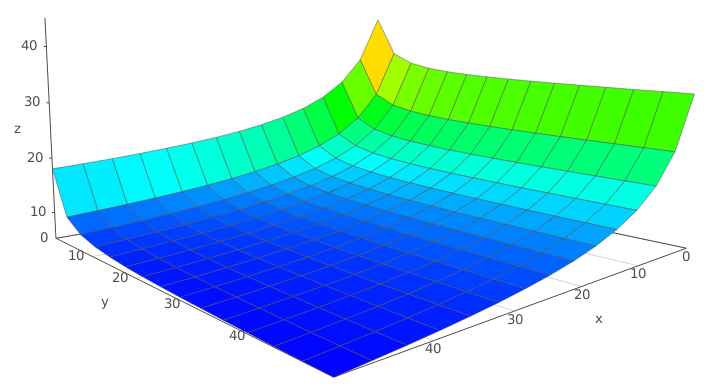
\includegraphics[width=9cm]{kiww}
		\caption{Gràfica de la funció $h_f(x,y,h_0)$ per $h_0=45$ i fent variar $x$ i $y$, on $x$ és el nombre de professors que pugen per l'assignatura i $y$ el preu en $kiwis$ que ha pagat el guanyador de la puja.}
		\label{fig:444}
	\end{figure}

\subsubsection{Assignacions finals}

Amb aquesta nova revalorització horària, es repartiran les matèries no assignades mitjançant el mètode de la funció entre els professors que tinguin de moment cobert un valor inferior a $\frac{2M}{3}$ hores, on M són les hores que ha de realitzar aquell professor.
\subsection{Subhastes condicionals i n-dimensionals}
\subsubsection{Problemàtiques de les  subhastes}
\begin{figure}
	\centering
	
\includegraphics[width=4cm]{eps}
	\caption{En aquesta figura veiem una icona del format d'arxiu \texttt{.eps}}
	\label{fig:3}
\end{figure}
Aquí tenim un resum de les problemàtiques que ha de soluciona el model de subhasta que considerem construir 
\begin{tcolorbox}[colback=black!1,title=\textbf{Llista problemàtiques subhastes},coltitle=black,colbacktitle=black!10]
\begin{enumerate}
	\item Les subhastes seran \textbf{seqüencials} o \textbf{simultànies}? Ja que les simultànies  poden implicar un \textbf{bloqueig de moneda} i les seqüencials poden implicar la inviabilitat de les \textbf{sol·licituds condicionals} i \nehh{no recordo}, almenys \textit{ a priori}.
	\item Com assignem les assignatures que no ha sol·licitat ningú?
	\item Les situacions de condicionals, com ara la puja de fer una assignatura condicionada a si  és compleix una condició.{\color{gray} Per exemple impartir amb un docent amb qui es té  \textit{bon tracte}, o bé tenir interès en un conjunt d'assignatures com a global i no per separat, és a dir, per conveniència horària} 
	\item Cas pràctic. Elegir assignatures per conveniència horària més  que per preferència de la matèria a impartir, sota la suposició de ser un criteri raonable i \textit{comú} en les dades històriques. {\color{gray} Per exemple voler impartir classe el menor nombre de dies per dificultats en el transport.}  
	\item Tot sistema que incentivi a mentir afavorira la especulació que farà poc \textbf{eficient} l'assignació final.
	\item Una assignació \textbf{optima} en tot cas haurà de  minimitzar la diferencia entre les \textbf{hores reals} i les \text{hores ideals}.
	\item Com desitgem una \textbf{revaloració} \footnote{Que pot ser la mateixa o no.} de cada matèria docent subhastada assumim que ha de ser necessari que la subhasta influeixi en el valor final de cada assignatura, en principi el valor en hores s'haurà de modificar.
	\item Situació de empat. {\color{gray} En cas de \textbf{subhasta simultània} .}
\end{enumerate}
\end{tcolorbox}
\subsubsection{Construcció primer model}
De forma constructiva, i aprofitant la subsecció prèvia, construirem un model que compleixi les condicions  de la llista anterior.

\subsubsection{Model de subhastes condicionals}
% Porque hitlur solo queria pintar cuadros
\begin{itemize}
	\item Subhastes multidimensionals en que es tenen en compte diverses coses per a decidir el guanyador de la subhasta
	\item Els professors poden fer pujes condicionades sobre els resultats d'altres subhastes
	\item Al finalitzar subhastes els seus resultats són propagats a altres subhastes passades on hi havia pujes condicionades sobre el resultat de la subhasta actual -> Subhastes passades actualitzen el seu resultat i el propaguen.
	\item Realitzem subhastes -> Eliminem assignacions que sobrepassin hores -> Realitzem subhastes -> ...
\end{itemize}

Algorisme
\begin{enumerate}
	\item Els professors entren totes les seves puges (que poden estar condicionades sobre altres pujes)
	\item Executar totes les subhastes una rer l'altra. En cas de trobar un apuja condicionada sobre una subhasta que no s'ha executat es considera la puja com a bona i s'executa la subhasta com si fos una puja normal, depsrés es fa una anotació marcant que aquesta puja depén de els resultats futurs d'una altra subhasta futura. Quan l'altra subhasta s'executi, al obtenir els resultats es revisita la subhasta depenent i, en cas que la puja condicional ja no sigui vàlida, aquesta subhasta és tornar a executar ignorant la puja invalidada. Aquestes invalidacions es propaguen sobre totes les subhastes depenents.
	\item Buscar els professors als que els hi ha sigut assignat assignatures que superen el nombre d'hores que haurien de realitzar, desassignar-lis suficients assignatures com per a que el nombre d'hores totals de les assignatures assignades a ells sigui semblant al nombre d'hores que han de fer. A continuació, aquests professors, les seves pujes i les assignatures que encara tenen assignades són eliminats del sistema.
	\item Si en el pas anterior s'han eliminat professors del sistema tornar al pas 2. En cas contrari, ja hem acabat i l'assignació final ja està feta (queda assignar les asisgnatures que no ha volgut ningú i vigilar que no hi hagi professors que hagin quedat amb molt poques assignatures assignades)
\end{enumerate}
ñ
\\
\newpage

%%%%%%%%%%%%%%%%%%%%%%%%%%%%%%%%%%%%%%%%%%%%%%%%%%%%
%                                                 %%
%    #06_1     Criteris o dades recopilació       %%
%                                                 %%
%%%%%%%%%%%%%%%%%%%%%%%%%%%%%%%%%%%%%%%%%%%%%%%%%%%%
\section*{Apèndix}
\begin{enumerate}
	\item \textbf{Paràmetres a optimitzar } (com a criteris) 
	\begin{itemize}
		\item La diferencia entre el nombre d'hores que \textit{hauria de fer} un professor i les hores que \textit{finalment farà} ha de ser el més petita possible. {\color{gray} Considerem que és l'estat més ideal.} \textbf{(minimitzar)} 
		\item La quantitat d'assignatures assignades a cada professors ha de ser baixa. 
		{\color{gray}  Per evitar el cas de que part del professorat tingui un nombre elevat de matèries a impartir, malgrat contin poc cadascuna ja que puntualment és pot tenir un sobrevolem de treball.} \textbf{(minimitzar)}
		\item L'assignació de les assignatures entre el professorat s'hauria d'acostar el màxim possible a les sol·licituds particulars demandades. {\color{gray}  L'elecció ja és justificació prou per argumentar que és una \textbf{alternativa} desitjable.} \textbf{(maximitzar)}
		\item S'hauria d'evitar que el nombre total d'hores de classe al dia d'un professor superés certs límits per a tots els dies.
		\item Les assignatures assignades a un mateix professor han de tenir certa localitat temporal, és a dir, que hi hagi poca diferència temporal entre el final d'una i el començament de la següent.
%{\color{gray} El motiu d'aquesta mesura és incentivar al professorat a invertir (opcionalment) en l'elaboració de material docent que malgrat el primer any de docencia li comporti un mayor esforç a la llarga sigui compensat, a més de millorar la docencia és clar.}
	\end{itemize}
    \item \textbf{Restriccions} (com a criteris)
    \begin{itemize}
    	\item No pot haver solapament d'hores entre les assignatures que ha d'impartir un mateix docent . {\color{gray} En essència això evita entre d'altres coses que un mateix docent hages d'estar a dos llocs diferents al'hora .} \textbf{(Restricció de existència)} 
    	\item El interval de temps entre el final d'una sessió de treball i el inici d'una altre, impartides per un mateix professional docent, a diferents facultats ha de ser major o igual a 20 minuts. {\color{gray} Un model que no contemples la pèrdua de temps en efectuar desplaçaments físics difícilment serà eficient i probablement precari.} \textbf{(Restricció d'ordre)} 
    	\item Les assignatures dels graus:
    	\begin{enumerate} 
    		\item Grau de Matemàtiques.
    		\item Grau d'Estadística Aplicada.
    		\item Grau de Matemàtica Computacional i Analítica de Dades.
    	\end{enumerate}
      No podran ser impartides pel mateix docent durant més de tres anys seguits.
      {\color{gray} Aquesta restricció té justificació per imposició de dades històriques i pràctiques.} \textbf{(Restricció d'ordre)} 
    	\item  . {\color{gray} .} \textbf{(minimitzar)} 
    	\item La resta d'assignatures dels vint-i-sis graus restants estarà limitada a quatre anys seguits de docència per un mateix docent. {\color{gray} Això per una banda implica un compromís de cara a la matèria impartida per cada docent, i per altra banda garanteix una estabilitat en el temari impartit de cara als estudiants.} \textbf{(Restricció d'ordre)} 
    	\item  Les matèries  dels cursos tercer i quart impartides als tres graus propis del departament \footnote{Grau de Matemàtiques, grau d'Estadística Aplicada, grau de Matemàtica Computacional i Analítica de Dades}. Sols podran ser impartides per docents que pertanyin a la unitat/subdepartament més proper a la matèria.   {\color{gray} La justificació és prou raonable, donada la actual \textit{especificació} inherent a la ciència en la actualitat. Un exemple seria que l'assignatura de Topologia sols pot ser impartida per docents de \textit{l'unitat} o \textit{subdepartament} de Geometria i Topologia \footnote{Veure secció de  \textit{model actual}.} .} \textbf{(Restricció d'ordre)} 
    \end{itemize}																								
%%%%%%%%%%%%%%%%%%%%%%%%%%%%%%%%%%%%%%%%%%%%%%%%%%%%
%                                                 %%
%    #07            Conclusions                   %%
%                                                 %%
%%%%%%%%%%%%%%%%%%%%%%%%%%%%%%%%%%%%%%%%%%%%%%%%%%%%
\begin{tcolorbox}[colframe=white,colback=redviolet!20,sharp corners=all,size=minimal,halign=center,valign=center]
	\section{Conclusions}
\end{tcolorbox}
\end{enumerate}
Dogmes de criteris
%%%%%%%%%%%%%%%%%%%%%%%%%%%%%%%%%%%%%%%%%%%%%%%%%%%%
%                                                 %%
%    #06_2   	       Bibliografia 	          %%
%                                                 %%
%%%%%%%%%%%%%%%%%%%%%%%%%%%%%%%%%%%%%%%%%%%%%%%%%%%%
\footnotesize
\bibliographystyle{ieeetr}
\bibliography{Bib.bib}
\end{document}
%https://youtu.be/mANIqat5IC8
